\documentclass[12pt]{article}
\usepackage{graphicx} % Required for inserting images
\usepackage{amsmath, amssymb}
\usepackage{tikz}
\usetikzlibrary{arrows.meta, positioning}
\usepackage{subfig}
\usepackage[round]{natbib}
\usepackage[margin = 2.5cm]{geometry}
\usepackage{url}
\usepackage{xr}
\externaldocument{appendix}

%\title{Deriving Complete Constraints in Hidden Variable Models}
%\author{Michael C.~Sachs \and Erin E.~Gabriel  \and Robin J.~Evans \and Arvid Sjölander}
%\date{\today}

\newcommand\indep{\protect\mathpalette{\protect\independenT}{\perp}}
\def\independenT#1#2{\mathrel{\rlap{$#1#2$}\mkern2mu{#1#2}}}

\newtheorem{proposition}{Proposition}
\newtheorem{definition}{Definition}
\newtheorem{example}{Example}
\newtheorem{condition}{Condition}
\newtheorem{remark}{Remark}

\def\Pr{{\mathrm{P}}}
\def\Pdo{{\mathrm{P}^*}}

\DeclareMathOperator{\Anobs}{Anobs}
\DeclareMathOperator{\Paobs}{Paobs}
\DeclareMathOperator{\Chobs}{Chobs}
\DeclareMathOperator{\Disobs}{Disobs}



\tikzset{rv/.style={circle, draw, inner sep=0.5mm, minimum size=7mm}}
\tikzset{fv/.style={draw}}

\newcommand{\bW}{\boldsymbol{W}}
\newcommand{\bU}{\boldsymbol{U}}
\newcommand{\bV}{\boldsymbol{V}}
\newcommand{\bR}{\boldsymbol{R}}
\DeclareMathOperator{\Do}{do}
\DeclareMathOperator{\Pa}{Pa}
% \DeclareMathOperator{\Do}{\mbox{do}}
% \DeclareMathOperator{\Pa}{\mbox{Pa}}

\setcounter{MaxMatrixCols}{20}

\def\spacingset#1{\renewcommand{\baselinestretch}%
{#1}\small\normalsize} \spacingset{1}
\newcommand{\blind}{0}

%\usepackage{setspace}
%\doublespacing

\begin{document}


\if1\blind
{
  \title{\bf Deriving Complete Constraints in Hidden Variable Models}
  \author{Michael C. Sachs$^1$\thanks{EEG and MCS are funded in part by NNF Grant NNF22OC0076595 and the Pioneer Centre for SMARTbiomed}, Erin E. Gabriel$^1$, \\
  Robin J. Evans$^2$,
  Arvid Sj\"olander$^3$\\  
\footnotesize 1:Section of Biostatistics and the Pioneer Centre for SMARTbiomed, \\ \footnotesize University of Copenhagen, Copenhagen, Denmark \\
\footnotesize 2:Department of Statistics, University of Oxford, Oxford, United Kingdom \\
\footnotesize 3:Department of Medical Epidemiology and Biostatistics, Karolinska Institutet, Stockholm, Sweden \\
\footnotesize corresponding author: michael.sachs@sund.ku.dk}
  \maketitle
} \fi 

\if0\blind
{
  \bigskip
  \bigskip
  \bigskip
  \begin{center}
    {\LARGE\bf Deriving Complete Constraints in Hidden Variable Models}
\end{center}
  \medskip
} \fi

\bigskip


\begin{abstract}
Hidden variable graphical models can sometimes imply constraints on the observable distribution that are more complex than simple conditional independence relations. These observable constraints can falsify assumptions of the model and can be used to constrain estimation procedures to improve statistical efficiency. Knowing the complete set of observable constraints is thus ideal, but this can be difficult to determine in many settings.  In models with categorical observed variables and a joint distribution that is completely characterized by linear relations to the unobservable response function variables, we develop a systematic method for deriving the complete set of observable constraints. We illustrate the method in several new settings, including ones that imply both inequality and equality constraints. \\
\noindent \textit{Keywords:} Causal models, Hidden variables, Constraints, Directed acyclic graphs.
\end{abstract}

\newpage
\spacingset{2}
\vspace{-1cm}

\section{Introduction}


The assumption of a structural model with hidden variables can rule out particular joint distributions not only due to observable conditional independence relations but also due to more complex observable conditions, which may not be clear from inspection of the causal model alone. These observable constraints can be used to falsify a structural model in settings where the data contradict these constraints. The instrumental inequalities first discussed in \citet{pearl1995testability} for the all binary instrumental variable (IV) setting are the most well-known example of these more complex constraints in the form of inequalities, while the ``Verma" constraints \citep{verma2022equivalence} are a well-known example of observable and thus falsifiable equality constraints representing a more general notion of conditional independence. 

In the general IV setting, \citet{bonet2001instrumentality} derived inequality constraints showing that, in cases with an IV with more than two categories, there are more observable constraints beyond the binary IV constraint set. Within the specific setting of all discrete observed variables within the classical trivariate IV setting he developed a method for deriving constraints on the observed data distribution implied by the causal assumptions and proved that these are the ``sufficient" set of constraints. We will use the term ``complete'' to refer to what \citeauthor{bonet2001instrumentality} called sufficient, but the meaning remains the same, i.e.~all observable and therefore falsifiable constraints implied by a structural model.  

The \citet{bonet2001instrumentality} method is what \citet{evans2012graphical} called the ``computationally intensive linear programming technique''. As pointed out by \citet{evans2012graphical}, complete constraints are difficult to derive without using such techniques or algebraic variable elimination algorithms, e.g., Fourier-Motzkin elimination, which become infeasible for moderately sized state spaces. Although other attempts have been made, such as \citet{kang2006inequality}, the derived constraints are not complete. This is also true for the \emph{nested Markov} characterization which, by construction, only involves equality constraints \citep{evans2019smooth, shpitser2012parameter, verma2022equivalence, richardson2023nested}.

We conceptually extend the method of \citet{bonet2001instrumentality} beyond the IV setting, which due to increased computational power is now feasible in many more settings. We prove that within the class of models that we refer to as ``linear", as defined in \citet{duarte2023automated}, our method provides the complete set of observable constraints. Linear here refers to settings with categorical observed variables and a joint distribution that is completely characterized by linear relations to the unobservable response function variables \citep{balke1994counterfactual, sachs2023general}. We also show that for the class of models for which our method provides complete constraints, the fully characterized joint distributions are a subclass of the distributions characterized by the nested Markov model in the same setting. In addition, we show that the proposed method can be used outside the ``linear" class to derive at least some of the constraints. We illustrate our method in several examples, providing, to our knowledge, novel constraints. All proofs are in the Appendix, Section \ref{appendix:proofs}, and software implementing the method is publicly available on GitHub at \url{https://github.com/sachsmc/meraconstraints}.



\section{Notation and Preliminaries}
\subsection{Notation}
Let $\mathcal{G}(\bV, \bU)$ be a hidden variables directed acyclic graph (DAG) representing a nonparametric structural equations model (NPSEM) \citep{Pearl2000causality}, over variables $\bW = \bV \cup \bU$ where $\bU$ are unobserved and $\bV$ are observed. We assume that all variables in $\bV$ are discrete and finite, but no assumptions are made about $\bU$. We will write $\bV_i$ (or some other index) to denote a subset of $\bV$, and $V_i$ a single element of $\bV$. Let $|\bV|$ denote the cardinality of the set $\bV$, and when used for a single variable, for example $|V_i|$, let it denote the number of possible values that variable $V_i$ can take, i.e., the cardinality of its domain. Let $\Paobs(\bV_i)$ denote the union of the sets of observed parents of each variable in the set $\bV_i$ and $\Pa(\bV_i)$ denote the union of the sets of all, observed or unobserved, parents of each variable in the set $\bV_i$. Let $\Anobs(\bV_i)$ denote the union of the sets of observed ancestors of each variable in $\bV_i$, where, as in \citet{evans2019smooth}, $V_2$ is an ancestor of $V_1$ if there is a sequence of directed edges $V_2 \rightarrow \cdots \rightarrow V_1$, and by definition, we include $V_1$ itself in the set of ancestors. Let $\Chobs(\bW_i)$ be the union of the sets of observed children of variables in $\bW_i$, where $W_1$ is a child of $W_2$ if and only if $W_2$ is a parent of $W_1$. 

\subsection{Settings}
Our goal is to characterize the distribution $\Pr(\bV)$, known as the marginal model (because it is marginal with respect to $\bU$), in terms of constraints implied by the NPSEM for $(\bV,\bU)$. Following \citet{evans2016graphs}, Section 3.2, we can restrict our attention to a smaller class of hidden variables DAGs that satisfy the following two conditions. In particular, it suffices to consider DAGs where none of the unobserved variables have parents, and where all of the unobserved variables have at least two observed children. 

\begin{condition} \label{A1}
All unobserved variables are exogenous, i.e., $\Pa(U_i) = \emptyset$ for all $U_i \in \bU$.
\end{condition}

\begin{condition} \label{A2}
The child set of each unobserved variable corresponds to a distinct
set of observed vertices of at least size 2. That is, for each $U_i \in \bU$, $|\Chobs(U_i)| \geq 2$, $\Chobs(U_i) \subseteq \bV_i$, and there is no $U_j \in \bU$ such that $\Chobs(U_i) \subseteq \Chobs(U_j)$.
\end{condition}

By Lemmas 1--3 of \citet{evans2016graphs}\footnote{Here we use the references to the published version of these Lemmas, rather than the arXiv version. The arXiv versions are Lemmas 3.7--3.9.}, DAGs where these conditions do not hold can be transformed to DAGs where they do hold without changing the implied marginal model. Briefly, the exogenization process replaces sequences of the form $W_1 \rightarrow U_1 \rightarrow V_1$ by $W_1 \rightarrow V_1$ without changing the marginal model, where $W_1$ could be observed or unobserved. Following exogenization, any unobserved variable $U_1$ whose child set is a subset of another unobserved variable $U_2$ can be absorbed into a common unobserved variable with child set equal to the union of child sets of $U_1$ and $U_2$. Examples of these transformations are given in the Appendix, Section \ref{appendix:trans}.



\begin{definition} \label{def:districts}
Let $\mathcal{G}(\bV, \bU)$ be a hidden variables DAG that by construction obeys Conditions \ref{A1} and \ref{A2}. Remove all edges that do not originate from variables in $\bU$. The sets of variables in $\bW$ that remain connected form a partition of $\bW$ called \emph{districts}. Denote $\mathcal{D}(\mathcal{G}) = \{D_1, \ldots, D_k\}$ the set of districts of $\mathcal{G}$. 
\end{definition}

This same concept is called a \emph{c-component} (short for confounded component) by \citet{tian2002testable}, while the term district is used in, e.g., \citet{richardson2003admgs}, \citet{evans2018margins}, and \citet {duarte2023automated}, which we will follow. We further define the c-degree of a district as follows.


\begin{definition}\label{def:cdeg}
Let $\mathcal{G}(\bV, \bU)$ be a hidden variables DAG that follows Conditions \ref{A1} and \ref{A2}. Let $D_j$ be a district in $\mathcal{G}(\bV, \bU)$. The \emph{c-degree} of $D_j$ is the number of hidden variables $U_i$ in $\bU$ that are in $D_j$. The c-degree of a DAG $\mathcal{G}(\bV, \bU)$ is the maximum of the c-degrees of its districts. 
\end{definition}

The example in Figure \ref{fig:district} illustrates the two definitions in this Section. The graph has three districts, one with c-degree 0 ($\{G\}$), one with c-degree 1 ($\{A, C, E, U_2\}$) and one with c-degree 2 ($\{B, D, F, U_1, U_3\}$). Thus, Figure \ref{fig:district} has c-degree 2. 



\begin{figure}[ht]
\begin{center}
  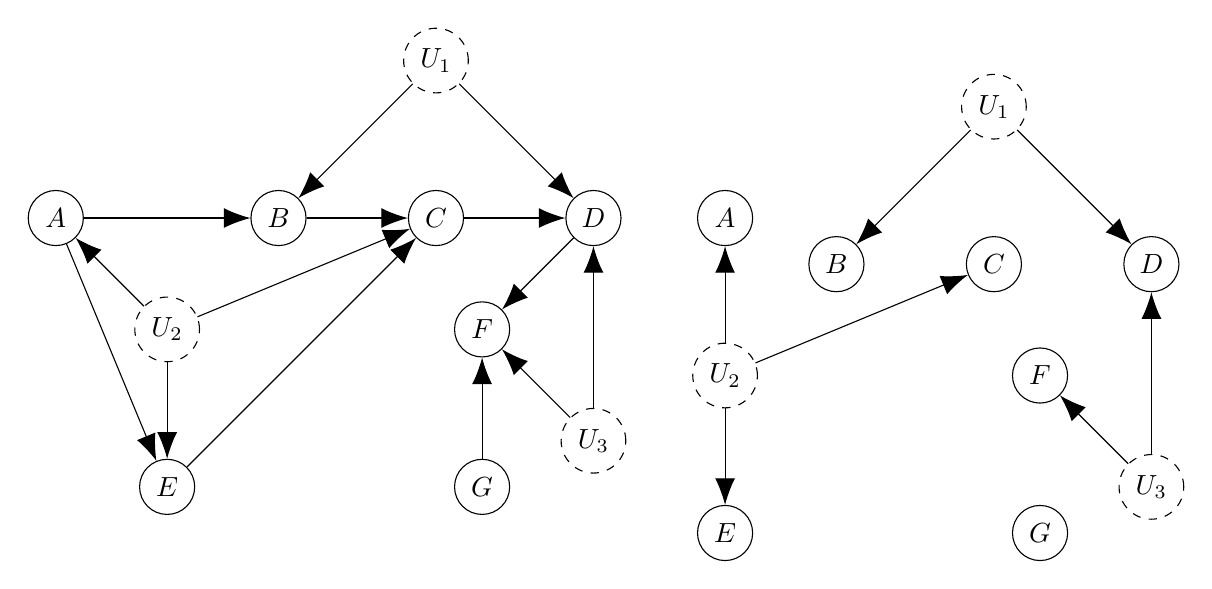
\begin{tikzpicture}[>=Stealth, node distance=2cm, on grid, auto]
\begin{scope}
  % Nodes
  \node (A) [rv] {$A$};
  \node[draw, circle, dashed] (U2) [below right= of A] {$U_2$};
  \node (B) [above right=of U2, rv] {$B$};
  \node (C) [right=of B, rv] {$C$};
  \node (D) [right=of C, rv] {$D$};
  
  \node (F) [below left=of D, rv] {$F$};
  \node (G) [below= of F, rv] {$G$};

  % unobserved variables (U1, U2, U3)
  \node[draw, circle, dashed] (U1) [above =of C] {$U_1$};
  
  \node[draw, circle, dashed] (U3) [below right=of F] {$U_3$};
\node (E) [below=of U2, rv] {$E$};
  % Arrows
  \draw [-{Latex[scale=2.0]}]  (A) -- (B);
  \draw [-{Latex[scale=2.0]}]  (E) -- (C);
  \draw [-{Latex[scale=2.0]}]  (C) -- (D);
  \draw [-{Latex[scale=2.0]}]  (D) -- (F);
  \draw [-{Latex[scale=2.0]}]  (A) -- (E);
  \draw [-{Latex[scale=2.0]}]  (B) -- (C);
  \draw [-{Latex[scale=2.0]}]  (G) -- (F);

  % Dashed arrows (unobserved variables)
  \draw [-{Latex[scale=2.0]}] (U1) -- (B);
  \draw [-{Latex[scale=2.0]}] (U1) -- (D);
  \draw [-{Latex[scale=2.0]}] (U2) -- (A);
  \draw [-{Latex[scale=2.0]}] (U2) -- (E);
  \draw [-{Latex[scale=2.0]}] (U2) -- (C);
  \draw [-{Latex[scale=2.0]}] (U3) -- (F);
  \draw [-{Latex[scale=2.0]}] (U3) -- (D);
    
\end{scope}
\begin{scope}[xshift = 8.5cm]
\node (A) [rv] {$A$};
  \node[draw,circle,dashed] (U2) [below= of A] {$U_2$};
  \node (B) [above right=of U2, rv] {$B$};
  \node (C) [right=of B, rv] {$C$};
  \node (D) [right=of C, rv] {$D$};
  
  \node (F) [below left=of D, rv] {$F$};
  \node (G) [below= of F, rv] {$G$};

  % unobserved variables (U1, U2, U3)
  \node[draw,circle,dashed] (U1) [above =of C] {$U_1$};
  
  \node[draw,circle,dashed] (U3) [below right=of F] {$U_3$};
\node (E) [below=of U2, rv] {$E$};
  % Dashed arrows (unobserved variables)
  \draw [-{Latex[scale=2.0]}] (U1) -- (B);
  \draw [-{Latex[scale=2.0]}] (U1) -- (D);
  \draw [-{Latex[scale=2.0]}] (U2) -- (A);
  \draw [-{Latex[scale=2.0]}] (U2) -- (E);
  \draw [-{Latex[scale=2.0]}] (U2) -- (C);
  \draw [-{Latex[scale=2.0]}] (U3) -- (F);
  \draw [-{Latex[scale=2.0]}] (U3) -- (D);
      
\end{scope}
\end{tikzpicture}
\end{center}
\caption{Example to illustrate Definitions \ref{def:districts} and \ref{def:cdeg}. The left figure is the original one, and the right figure has the edges originating from observed variables removed. The graph has three districts: $\{G\}$ with c-degree 0, $\{A, C, E, U_2\}$ with c-degree 1, and $\{B, D, F, U_1, U_3\}$ with c-degree 2. \label{fig:district}}
\end{figure}

\clearpage


\subsection{Canonical partitioning} \label{sec:respvar}

A DAG that follows Conditions \ref{A1}, \ref{A2}, and that has a c-degree of 1 comprises districts of either singleton observed variables or sets of observed variables that all share a single common unobserved parent. Such DAGs can be transformed into equivalent mixed graphs (containing directed and undirected edges) that remove unobserved variables $\bU$ having arbitrary distribution and replaces them with a set of unobserved variables $\boldsymbol{R}$ that are categorical. These are called \emph{response function variables} by \citet{balke1994counterfactual} and \emph{selectors} by \citet{bonet2001instrumentality}. This is possible because each observed variable is categorical, which induces a canonical partitioning \citep{Pearl2000causality}. See also Theorem 1 of \citet{sachs2023general}. 

\begin{definition}
Let $\mathcal{G}(\bV, \bU)$ be a hidden variables DAG that follows Conditions \ref{A1}, \ref{A2}, and has a c-degree of 1. The \emph{response variable transformation} of $\mathcal{G}(\bV, \bU)$ is a mixed graph $\mathcal{G}(\bV, \bR)$ where: 
\begin{itemize}
    \item for each $V_i \in \bV$, introduce a new unobserved variable $R_{V_i}$ that is discrete with $|V_i|^{k_i}$ levels, where $k_i = \prod_{V \in \Paobs(V_i)}|V|$, and add an edge $R_{V_i} \rightarrow V_i$; 
    \item introduce an undirected edge $R_{V_i} \text{---} R_{V_j}$ for every pair of variables $V_i, V_j$ that are in the same district.
\end{itemize}
\end{definition}

The value of $R_{V_i}$ determines the way that $V_i$ responds to its parents. The undirected edges that connect $R_{V_i}$ and $R_{V_j}$ indicate a statistical dependence, so that $\Pr(R_{V_i} = a, R_{V_j} = b) = \Pr(R_{V_i} = a)\Pr(R_{V_j} = b)$ if $R_{V_i}$ and $R_{V_j}$ are not connected by a undirected edge, but $\Pr(R_{V_i} = a, R_{V_j} = b)$ is not necessarily equal to $\Pr(R_{V_i} = a)\Pr(R_{V_j} = b)$ if they are connected. An example is shown in Figure \ref{fig:seqiv}. We will refer to $R_{V_i}$ as the response function variable of $V_i$, and use the notation $\boldsymbol{R}_{\bV_i}$ to denote the vector of response function variables for the vector of observed variables $\bV_i$. Response function variables will be connected within a district, but never between different districts. 

\begin{figure}[ht]
\centering
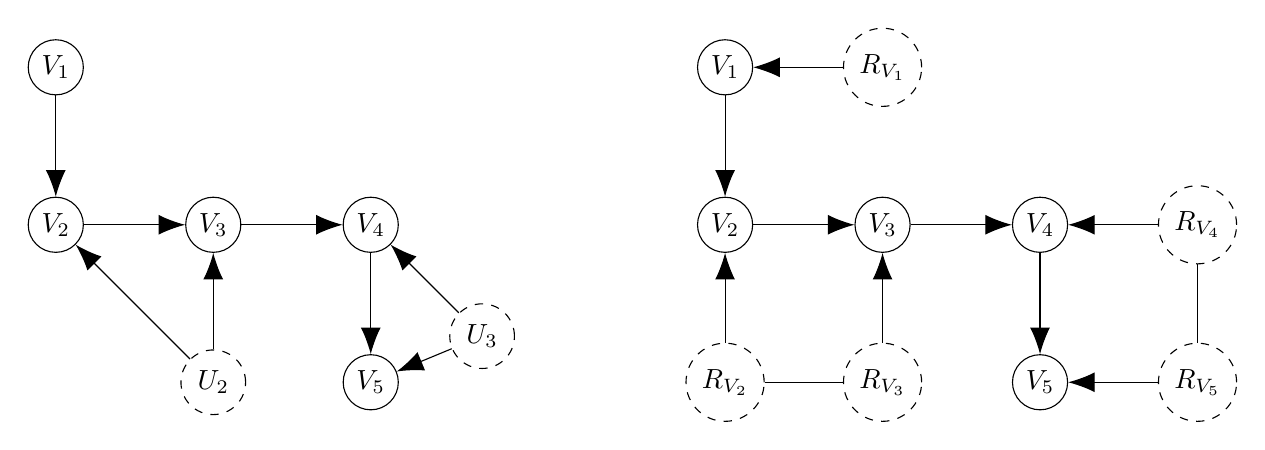
\begin{tikzpicture}[>=Stealth, node distance=2cm, on grid, auto]

  \begin{scope}
  \node (V1) [rv] {$V_1$};
  \node (V2) [below = of V1, rv] {$V_2$};
  \node (V3) [right = of V2, rv] {$V_3$};
  \node (V4) [right = of V3, rv] {$V_4$};
  \node (V5) [below = of V4, rv] {$V_5$};
  %\node (U1) [right = of V1] {$U_1$};
  \node[draw, circle, dashed] (U2) [below = of V3] {$U_2$};
  \node[draw, circle, dashed] (U3) [below right = of V4] {$U_3$};
  
  
  % Arrows
  \draw [-{Latex[scale=2.0]}] (V1) -- (V2);
  \draw [-{Latex[scale=2.0]}] (V2) -- (V3);
  \draw [-{Latex[scale=2.0]}] (V3) -- (V4);
%  \draw [-{Latex[scale=2.0]}] (V3) -- (V5);
  \draw [-{Latex[scale=2.0]}] (V4) -- (V5);
  
  % Dashed arrows (unobserved variables)
  %\draw [-{Latex[scale=2.0]}] (U1) -- (V1);
  \draw [-{Latex[scale=2.0]}] (U2) -- (V2);
  \draw [-{Latex[scale=2.0]}] (U2) -- (V3);
  \draw [-{Latex[scale=2.0]}] (U3) -- (V4);
  \draw [-{Latex[scale=2.0]}] (U3) -- (V5);
    
  \end{scope}% Nodes
  \begin{scope}[xshift=8.5cm]  % Nodes
  \node (V1) [rv] {$V_1$};
  \node (V2) [below = of V1, rv] {$V_2$};
  \node (V3) [right = of V2, rv] {$V_3$};
  \node (V4) [right = of V3, rv] {$V_4$};
  \node (V5) [below = of V4, rv] {$V_5$};
  \node[draw, circle, dashed] (RV1) [right = of V1] {$R_{V_1}$};
  \node[draw, circle, dashed] (RV2) [below = of V2] {$R_{V_2}$};
  \node[draw, circle, dashed] (RV3) [below = of V3] {$R_{V_3}$};
  \node[draw, circle, dashed] (RV4) [right = of V4] {$R_{V_4}$};
  \node[draw, circle, dashed] (RV5) [right = of V5] {$R_{V_5}$};
  
  % Arrows
  \draw [-{Latex[scale=2.0]}] (V1) -- (V2);
  \draw [-{Latex[scale=2.0]}] (V2) -- (V3);
  \draw [-{Latex[scale=2.0]}] (V3) -- (V4);
%  \draw [-{Latex[scale=2.0]}] (V3) -- (V5);
  \draw [-{Latex[scale=2.0]}] (V4) -- (V5);
  
  % Dashed arrows (unobserved variables)
  \draw [-{Latex[scale=2.0]}] (RV1) -- (V1);
  \draw [-{Latex[scale=2.0]}] (RV2) -- (V2);
  \draw [-{Latex[scale=2.0]}] (RV3) -- (V3);
  \draw [-{Latex[scale=2.0]}] (RV4) -- (V4);
  \draw [-{Latex[scale=2.0]}] (RV5) -- (V5);

  \draw[] (RV2) -- (RV3);
  \draw[] (RV4) -- (RV5);
\end{scope}
\end{tikzpicture}
\caption{A sequential instrumental variable example, and its response function variable transformation.\label{fig:seqiv}}
\end{figure}

\begin{remark} \label{rmk1}
Let $\mathcal{G}(\bV, \bU)$ be a hidden variables DAG that follows Conditions \ref{A1}, \ref{A2}, and has a c-degree of 1. The response variable transformation of $\mathcal{G}(\bV, \bU)$ results in the same structural model, i.e. the same values of all variables under any intervention (including no intervention) on any of the observed variables in the DAG. 
\end{remark}

The response function variable transformation preserves the marginal model, and also allows us to exploit the discreteness of the observations to formulate a set of linear constraints. Given a value of a response function variable, say $R_{V_i} = b$, there exists a response function $f_{V_i}^b(\Paobs(V_i))$ that determines an observed value for $V_i$ given $\Paobs(V_i)$. So $f_{V_i}^b: \operatorname{domain}(\Paobs(V_i)) \rightarrow \operatorname{domain}(V_i)$. Given values of the response function variables for $V_i$ and all of its ancestors, the value of $V_i$ is determined by recursive substitutions \citep{sachs2023general, duarte2023automated}. Therefore we can write all observable probabilities and interventional probabilities in terms of probabilities of response function variables. Following \citet{tian2002testable}, we will call the equations relating these two forms of probabilities \emph{functional constraints}. 


\subsection{Functional constraints}

An algorithm and implementation to obtain the set of functional constraints for DAGs that fit a more strict set of criteria than what we consider here was presented in Algorithm 1 of \citet{sachs2023general}. A more general algorithm for settings with arbitrary c-degree is presented in \citet{duarte2023automated}, where the constraints are polynomials. Their Proposition 4 states that the degree of the polynomial constraints is bounded above by the c-degree of the corresponding district. In our next Proposition we explicitly relate the functional constraints to observable probabilities, forming the foundation of the observable constraint derivation.


\begin{proposition} \label{prop:ident}
Suppose $\mathcal{G}(\bV, \bU)$ is a hidden variables DAG that follows Conditions \ref{A1} and \ref{A2}. Further, suppose $\bV_1$ is the vector of all observed variables in the district $D_1$, and let $\bV_2 = \Paobs(\bV_1) \setminus \bV_1$ be the vector of observed parents of $\bV_1$ that are not part of $\bV_1$. Order the variables in $\bV_1=(V_{11},\ldots,V_{1k})$ topologically,
and let $\bV_1^{<i}=(V_{11},\ldots,V_{1,i-1})$ and
$\bV_2^{(i)}=\bV_2\cap \Anobs(V_{1i})$.  Define
\[
    \Pdo(\bV_1=v_1\mid \bV_2=v_2)
    =
    \prod_{i=1}^k
    \Pr\!\left(
        V_{1i}=v_{1i}
        \,\middle|\,
        \bV_1^{<i}=v_1^{<i},
        \bV_2^{(i)}=v_2^{(i)}
    \right).
\]
If $D_1$ has c-degree 1, then for all possible values of the vectors $v_1 = (v_{11}, \ldots, v_{1k}), v_2 = (v_{21}, \ldots, v_{2\ell})$, the functional constraints on $\Pdo(\bV_1 = v_{1} |\bV_2 = v_2)$ under $\mathcal{G}(\bV, \bU)$ are linear functions of response function variable probabilities of $\mathbf{R}_{\bV_1}$.
\end{proposition}

Let $\Pr(\bV_1 = v_1 | \Do(\bV_2 = v_2))$ denote the joint probability of $\bV_1 = v_1$ under the intervention that sets $\bV_2 = v_2$. All of the $\Pdo(\bV_1 = v_{1} |\bV_2 = v_2)$ referenced in Proposition \ref{prop:ident} can be given a causal interpretation using the do operator, such that $\Pdo(\bV_1 = v_{1} |\bV_2 = v_2) =  \Pr(\bV_1 = v_{1} | \Do(\bV_2 = v_2))$. 

\begin{proposition} \label{causalprop}
Suppose $\mathcal{G}(\bV, \bU)$ is a hidden variables DAG that follows Conditions \ref{A1}, \ref{A2}, and $\bV_1$, $\bV_2$ are as described in Proposition \ref{prop:ident}. Then all $\Pr(\bV_1 = v_{1} | \Do(\bV_2 = v_2))$ are identified and given by $\Pdo(\bV_1 = v_1|\bV_2=v_2)$. 
\end{proposition}
We note that one could also consider similar counterfactual quantities, e.g., $\Pr(\bV_1(v_2)=v_1)$, rather than the do-operator interventional quantities and Proposition \ref{causalprop} would also hold.

Consider the example in Figure \ref{fig:ivclassic}, the left most of which is the classical IV setting. In this case there are 2 districts, $\{Z\}$ with c-degree 0 and $\{X, Y, U\}$ with c-degree 1, and Conditions \ref{A1} and \ref{A2} are satisfied. Letting $\bV_1 = (X, Y)$ and applying Proposition \ref{prop:ident} we have $\bV_2 = \Paobs(\{X, Y\}) \setminus \{X, Y\} = \{Z\}$, $\Anobs(Y) = \{X, Z\}$, $\Anobs(X) = \{Z\}$, and 
\begin{align*}
    \Pdo(\bV_1 = v_{1} |\bV_2 = v_2) &= \Pr(Y = y | X = x, Z = z) \Pr(X = x | Z = z)\\ 
    & = \Pr(X = x, Y = y | \Do(Z = z)) \\
    & = \sum_{b \in \mathcal{B}} \Pr((R_x, R_y) = b), \mbox{ for all } x, y, z,
\end{align*}
where $\mathcal{B} = \{(b_x, b_y): f^{b_y}_Y(f^{b_x}_X(z)) = y \mbox{ and } f^{b_x}_X(z) = x\}$ for the structural equations $f^{b_y}_Y$ and $f^{b_x}_X$. The series of functional constraints for each combination of values of $z, x, y$ can be represented by the matrix equation
\[
\boldsymbol{p_{xy\cdot z}} = \boldsymbol{B} \boldsymbol{r_{xy}}, 
\]
where, for binary $X, Y, Z$, $\boldsymbol{p_{xy\cdot z}}$ is the vector of 8 probabilities $[\Pr(Y = y | X = x, Z = z) \Pr(X = x | Z = z): x, y, z \in \{0, 1\}]$, $\boldsymbol{B}$ is an $8 \times 16$ matrix of 0s and 1s, and $\boldsymbol{r_{xy}}$ is the vector of 16 response function variable probabilities $[\Pr((R_x, R_y) = (b_x, b_y)): b_x, b_y \in \{0, 1, 2, 3\}]$.

\begin{figure}[ht]
\centering

    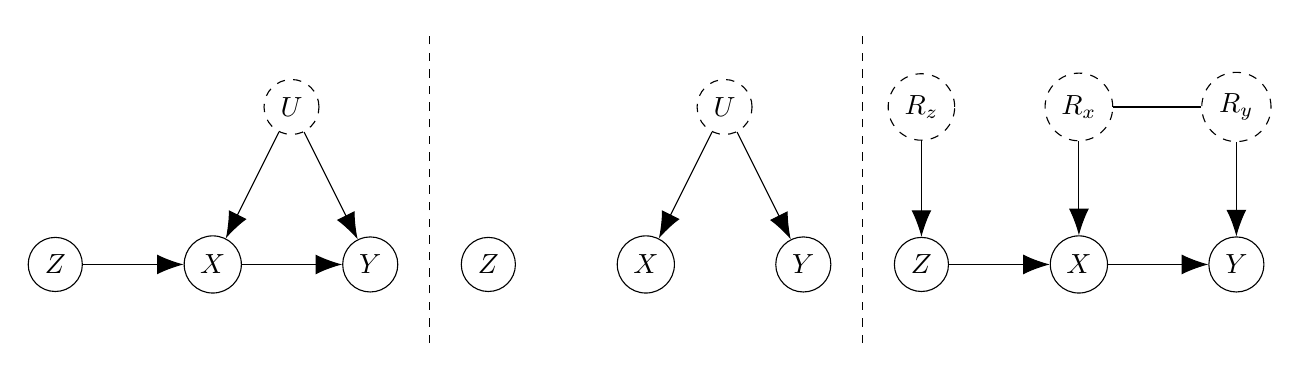
\begin{tikzpicture}
    \begin{scope}[xshift=-2cm]
    \node[draw, circle] at (2, 0) (X) {\(X\)};
    \node[draw, circle] at (4, 0) (Y) {\(Y\)};
    \node[draw, circle] at (0, 0) (Z) {$Z$};
    %\node[draw, circle] at (-3, 4) (S) {\(S\)};
   % \node[draw, circle] at (-4, 0) (Z) {\(Z\)};
    \node[draw, circle, dashed] at (3,2) (U) {\(U\)};
    \draw [-{Latex[scale=2.0]}] (X) to (Y);
    \draw [-{Latex[scale=2.0]}] (Z) to (X);
    %\draw [-{Latex[scale=2.0]}] (S) to (X);
    %\draw [-{Latex[scale=2.0]}] (S) to (Y);
    \draw [-{Latex[scale=2.0]}] (U) to (X);
    \draw [-{Latex[scale=2.0]}] (U) to (Y);
   % \draw [-{Latex[scale=2.0]}] (Z) to (X);
    %\draw [-, dashed] (S) to (U);
    \draw[dashed] (4.75, -1) -- (4.75, 3);

    \end{scope}% Nodes
\begin{scope}[xshift=3.5cm]
    \node[draw, circle] at (2, 0) (X) {\(X\)};
    \node[draw, circle] at (4, 0) (Y) {\(Y\)};
    \node[draw, circle] at (0, 0) (Z) {$Z$};
    %\node[draw, circle] at (-3, 4) (S) {\(S\)};
   % \node[draw, circle] at (-4, 0) (Z) {\(Z\)};
    \node[draw, circle, dashed] at (3,2) (U) {\(U\)};
  %  \draw [-{Latex[scale=2.0]}] (X) to (Y);
   % \draw [-{Latex[scale=2.0]}] (Z) to (X);
    %\draw [-{Latex[scale=2.0]}] (S) to (X);
    %\draw [-{Latex[scale=2.0]}] (S) to (Y);
    \draw [-{Latex[scale=2.0]}] (U) to (X);
    \draw [-{Latex[scale=2.0]}] (U) to (Y);
   % \draw [-{Latex[scale=2.0]}] (Z) to (X);
    %\draw [-, dashed] (S) to (U);
    \draw[dashed] (4.75, -1) -- (4.75, 3);

    \end{scope}% Nodes
    
  \begin{scope}[xshift=9cm] 
    
    \node[draw, circle] at (2, 0) (X) {\(X\)};
    \node[draw, circle] at (4, 0) (Y) {\(Y\)};
    \node[draw, circle] at (0, 0) (Z) {$Z$};
    %\node[draw, circle] at (-3, 4) (S) {\(S\)};
   % \node[draw, circle] at (-4, 0) (Z) {\(Z\)};
    \node[draw, circle, dashed] at (2,2) (Rx) {\(R_x\)};
    \node[draw, circle, dashed] at (4,2) (Ry) {\(R_y\)};
    \node[draw, circle, dashed] at (0,2) (Rz) {\(R_z\)};
    \draw [-{Latex[scale=2.0]}] (X) to (Y);
    \draw [-{Latex[scale=2.0]}] (Z) to (X);
    %\draw [-{Latex[scale=2.0]}] (S) to (X);
    %\draw [-{Latex[scale=2.0]}] (S) to (Y);
    \draw [-{Latex[scale=2.0]}] (Rx) to (X);
    \draw [-{Latex[scale=2.0]}] (Ry) to (Y);
    \draw [-{Latex[scale=2.0]}] (Rz) to (Z);
    \draw (Rx) -- (Ry);
   % \draw [-{Latex[scale=2.0]}] (Z) to (X);
    %\draw [-, dashed] (S) to (U);
  

  \end{scope}
    \end{tikzpicture}
  
    \caption{\label{fig:ivclassic} The instrumental variable DAG in original form (left), showing the two districts (center), and response variable form (right).}
    \end{figure}  

% Although we interpret the $\Pr(\bW_1 =w_1| \Do(\bW_2)=w_2)$ as causal, one does not need to do so. Instead, one can simply define $\Pr(\bW_1 =w_1| \Do(\bW_2)=w_2)$ to be a function that is given by:   
% \[
%     \prod_{i: W_{1i} \in D_1} \Pr(W_{1i} = w_{1i} | \{\Paobs(\bW_1) \cap \Anobs(W_{1i})\} \setminus W_{1i}).
% \]
% which allows one to equate $\Pr(\bW_1 =w_1| \Do(\bW_2)=w_2)$ with $Q_j$ in equation (29) of \citet{tian2002identification} without requiring a causal interpretation. The proof of Proposition \ref{prop:ident} then follows just as shown in the Appendix. 



\subsection{Nested Markov models}

The nested Markov models \citep{richardson2023nested} further constrain the state-space of these sets of distributions. Briefly put, they allow (generalized) conditional independence constraints to be encoded within a hidden variables DAG model, and in the discrete case to know that these independences are the only \emph{equality} constraints in the model \citep{evans2018margins}. 


While a regular conditional independence relation, for example $X \indep Y \mid Z$, can be expressed as $\Pr(X | Y, Z) = \Pr(X | Z)$, a \emph{nested Markov independence} is a more general statement about a lack of dependence of a quantity on a particular variable. In particular, the quantities in question are probabilities in graphs after removing arrows into certain variables (i.e., intervening on them). For example, they can be expressed as $\sum_B \Pr(D | A, B, C)\Pr(B | A) = g(D, C)$, for some function $g$; note the lack of dependence on $A$ here. Such relations are also sometimes called \emph{Verma constraints} after \citet{verma2022equivalence}, and \emph{post-truncation independences} after \citet{shpitser2012parameter}.
Further details are given in the Appendix, Section \ref{sec:nmm}.



\section{Method for deriving constraints and completeness results}

Given those preliminaries, we now detail our algorithm for deriving observable constraints in a hidden variables DAG with discrete and finite observed variables. To summarize briefly, we begin by using d-separation to list all conditional and marginal independencies implied by the DAG, if there are any. Then, for each district, ensuring that the c-degree of each district is 1, we derive the matrix equations representing the linear functional constraints by Proposition \ref{prop:ident}. These matrix equations describe the extreme points of a convex polyhedron in terms of the unobservable quantities involving probabilities of the response function variables. We can convert this to an equivalent description of the same convex polyhedron in terms of only observable quantities. This is called the vertex-to-halfspace (V-to-H) conversion, and different algorithms exist to efficiently perform this conversion that are implemented in open-source software programs such as \texttt{cddlib} \citep{cdd}. This is similar to the insight described in \citet{bonet2001instrumentality}, which was restricted to the instrumental variable setting.

\subsection{Description of the algorithm} \label{algorithm}


\textbf{Inputs: } A hidden variables DAG $\mathcal{G}(\bV, \bU)$ that meets Conditions \ref{A1}, \ref{A2} and has c-degree 1. 
\begin{enumerate}
    %\item Convert $\mathcal{G}'$ to the canonical DAG $\mathcal{G}$ using the Algorithm 1 of \citet{duarte2023automated}. 
   % \item Do the latent projection operation to get an ADMG $\mathcal{G}(\bV)$ \citep{verma2022equivalence}
    \item Enumerate the conditional independencies using a standard algorithm based on checking for d-separation, e.g., \citet{van2014constructing}, or using lines 1--8 of Algorithm 1 of \citet{richardson2023nested}.
    \item[] \, \textbf{Output: } List of standard independence constraints.  
    \item Identify the districts $\mathcal{D} = \{D_1, \ldots, D_M\}$. 
    \item Do the response function variable transformation of $\mathcal{G}$ into $\mathcal{G}^\dagger$ as described in Section \ref{sec:respvar}.
    \item For each district $D_j$: 
   \begin{enumerate}  
        \item Derive the formula for $\Pdo(\bV_1 = v_1 | \bV_2 = v_2)$, where $\bV_1$ are all the observed variables in $D_j$ and $\bV_2 = \Paobs(\bV_1) \setminus \bV_1$, using Proposition \ref{prop:ident}.
        \item For each combination of $v_1, v_2$, derive the functional probabilities, i.e., 
        \[
        \sum_{b \in \mathcal{B}} \Pr(\boldsymbol{R}_{\bV_1} = b), 
        \]
    where $\mathcal{B}$ is the set of response function variable values that are compatible with the observation vector $v_1, v_2$. 
    \item Construct the matrix representing the system of linear equations relating 
    \[
    \Pdo(\bV_1 = v_1 |\bV_2 = v_2) = \sum_{b \in \mathcal{B}} \Pr(\boldsymbol{R}_{\bV_1} = b) \Leftrightarrow \boldsymbol{p} = \boldsymbol{B} \boldsymbol{r}.
    \]
    \item Add a row of all 1s to $\boldsymbol{B}$ which represents the constraint that the response function variable probabilities all sum to 1. 
    \item Convert $\boldsymbol{p} = \boldsymbol{B} \boldsymbol{r}$ to the H-representation, e.g., using the double description method \citep{cdd, doubledescriptionmethod}.
    \item[] \, \textbf{Output: } The H-representation and the vector $\boldsymbol{p}$ of the formulae for $\Pdo(\bV_1 = v_1 |\bV_2 = v_2)$ for each district
    \end{enumerate}
\end{enumerate}

The H-representation consists of two rational matrices $H_i, H_e$ and rational vectors $b_i, b_e$ such that 
\[
H_i \boldsymbol{p} \leq b_i
\mbox{ and }
H_e \boldsymbol{p} = b_e. 
\]
In other words, it provides a representation of inequality and equality constraints in terms of the observable probability vector. 
These expressions encode both inequality and equality constraints. 

We apply the Algorithm to the second district of the binary IV example which contains $X$ and $Y$. The worked details are in the Appendix, Section \ref{appendix:iv}. For example, the 5th row of $H_i$ and corresponding element of $b_i$ encode the constraint
\[
\Pr(Y = 1, X = 0 | Z = 0) + \Pr(Y = 0, X = 0 | Z = 1) \leq 1,
\]
which is one of the classic instrumental inequalities as derived by \citet{pearl1995testability}. The equality constraints encoded by $H_e$ are simply the standard probabilistic constraints: 
\begin{equation}
\sum_{x, y \in \{0, 1\}} \Pr(Y = x, X = y | Z = z) = 1, \mbox{ for } z = 0, 1. \label{eqn:ivex}    
\end{equation}


\subsection{Completeness results} \label{sec:complete}



%\begin{definition}
%    A causal model $G$ is \emph{linear} if all distributions compatible with $G$ satisfy a linear system of functional constraints. 
%\end{definition}

%Thus, if a causal model is linear then the complete set of functional %constraints are linear. 

\begin{proposition} \label{prop:complete}
 Let $\mathcal{G}$ be a hidden variables DAG satisfying Conditions \ref{A1}, \ref{A2}, and having c-degree 1. Let $\mathcal{C}(\mathcal{G})$ be the set of observed distributions satisfying the conditional independencies implied by $\mathcal{G}$ and the district level H-representation constraints returned by the algorithm. Then
\[
    \mathcal{M}(\mathcal{G}) = \mathcal{C}(\mathcal{G}),
\]
where $\mathcal{M}(\mathcal{G})$ denotes the marginal model over the observed variables. Hence the constraints derived from the algorithm, together with the conditional independencies, are complete.
\end{proposition}

In other words, if every district in a DAG has at most one latent common cause, then the constraints derived by our algorithm are necessary and sufficient, i.e., the marginal model is exactly the set of observed distributions satisfying these constraints. This result stems from the linearity of the functional constraints, which means that we can then use standard results from computational geometry to convert them to observable constraints. The fact that the V- and H- representations are equivalent ensures nothing is lost from the V-to-H conversion which is the cornerstone of our approach to getting the observable constraints. The district factorization of the marginal distribution and our Proposition \ref{prop:ident} ensures that there are no components of the marginal distribution left unexamined. 

As a case where the Algorithm does not apply, consider the DAG in Figure \ref{fig:triangle}, left side, often referred to as the triangle scenario. The triangle scenario has c-degree 3, and comprises a single district. Our algorithm cannot be applied in this case, however, it is known that some observed probability distributions are incompatible with the triangle scenario. For example, \citet{Wolfe_2019} demonstrates that the distribution where $\Pr(A = 1, B = 1, C = 1) = \Pr(A = 0, B = 0, C = 0) = 1/2$ is incompatible with the triangle scenario. An additional example is the left side of Figure \ref{fig:incomp}. As discussed in Section \ref{sec:nonlin} and \ref{graphmod}, one can modify such graphs to obtain some or all constraints in some settings. 



\subsection{Identifying nontrivial constraints}


\begin{definition} \label{def:nontrivial}
    An observable constraint is \textbf{nontrivial} if it restricts the full joint distribution beyond the standard probabilistic constraints (i.e., probabilities sum to 1 and are between 0 and 1).  
\end{definition}


An example of an observable constraint is $\Pr(V_1 = v_1) \geq 0$, which is trivial because it is implied by the axioms of probability and not the structural model. Another example is given in Equation \eqref{eqn:ivex} in the illustration of our algorithm on the IV setting. We propose a simple procedure for identifying the subset of potentially nontrivial constraints from the output of our algorithm. It is based on the observation that the H-representations are linear constraints on a vector of probabilities, i.e., 
\[
H_i \boldsymbol{{p}} \leq b_i
\mbox{ and }
H_e \boldsymbol{{p}} = b_e,
\]
where $\boldsymbol{{p}} = [\Pdo(\bV_1 = v_1 |\bV_2 = v_2): \mbox{ for all possible values of } v_1, v_2]$. The unconstrained space of probabilities is the cross product of the probability simplices of the appropriate dimension, which is a convex polyhedron. Since the constraints are linear in these probabilities, violations can be witnessed at the extreme points of the unconstrained polyhedron. If these extreme points do not produce violations, the constraints are definitely trivial. Thus, our approach is to enumerate the extreme points of the unconstrained polyhedron, and then test if any of the derived constraints are ever violated at these points; violations identify potentially nontrivial constraints. We state this in the following proposition and illustrate it in the IV example. 


%Note that functional constraints on just joint probabilities from a single district never imply nontrivial observable constraints. 

\begin{proposition} \label{prop:nontrivial}
    Suppose $\mathcal{G}(\bV, \bU)$ is a hidden variables DAG that follows Conditions \ref{A1}, \ref{A2}, and with the H-representation of constraints on a given district from our Algorithm in Section \ref{algorithm} of the form
\[
H_i \boldsymbol{{p}} \leq b_i
\mbox{ and }
H_e \boldsymbol{{p}} = b_e,
\]
where $\boldsymbol{{p}} = [\Pdo(\bV_1 = v_1 |\bV_2 = v_2): \mbox{ for all possible values of } v_1, v_2]$.  Let $\boldsymbol{\check{P}}$ denote the cross-product of probability simplices, one for each unique value of $v_2$, in the order corresponding to $\boldsymbol{{p}}$. Any nontrivial constraints encoded by $H_i$ and $H_e$ are violated by at least one of the extreme points of  $\boldsymbol{\check{P}}$.
\end{proposition}

%Note (H-to-V) of a nontrivial observable constraint will result in an \textbf{informative counterfactual constraint.}
%\begin{proposition}
%    Given a DAG $G$, a probability of the form $\Pr(\bW_1 = w_1 |\Do(\bW_2 = w_2))$ emits a nontrivial linear observable constraint if $\bW_2$ is not empty. 
%\end{proposition}

The proposition gives a necessary condition for nontriviality of a row of the H-representation: rows that are never violated at the extreme points of $\boldsymbol{\check{P}}$ are trivial, while rows that are violated at some extreme point may still require manual simplification and inspection to confirm nontriviality.

Continuing with the IV example from the previous section and applying Proposition \ref{prop:nontrivial}, the $\boldsymbol{\check{P}}$ space is the cross-product of 2 probability simplices, one for $z = 0$ and one for $z = 1$. The extreme points are represented in the matrix $\boldsymbol{\check{P}}$ shown in the Appendix, Section \ref{appendix:iv}, where each row represents an instance of the vector 
\[
[\Pdo(0, 0 | 0), \Pdo(1, 0 | 0), \Pdo(0, 1 | 0), \Pdo(1, 1 | 0), \Pdo(0, 0 | 1), \Pdo(1, 0 | 1), \Pdo(0, 1 | 1), \Pdo(1, 1 | 1)]. 
\]
We then check whether $H_i \boldsymbol{\check{p}} > b_i$ or $H_e \boldsymbol{\check{p}} \neq b_e$ for each $\boldsymbol{\check{p}}$ in the rows of the above matrix. We find that the equality constraints are never violated, and the 2nd, 3rd, 5th and 6th rows of $H_i$ are violated by at least one of the extreme points. These constraints are (after some simple algebra) the classical instrumental inequalities: 
\begin{align*}
 & \Pr(Y = 1,X = 1|Z = 0) + \Pr(Y = 0,X = 1|Z = 1) \leq 1 \\
& \Pr(Y = 0,X = 1|Z = 0) + \Pr(Y = 1,X = 1|Z = 1)  \leq 1 \\
& \Pr(Y = 1,X = 0|Z = 0) + \Pr(Y = 0,X = 0|Z = 1) \leq 1 \\
& \Pr(Y = 0,X = 0|Z = 0) + \Pr(Y = 1,X = 0|Z = 1) \leq 1.  
\end{align*}
We can follow the same procedure for the other district which contains the singleton $Z$. However, singleton districts with no parents cannot give any nontrivial constraints, so we omit the details. 


We note that the algorithm identifies all nontrivial observable constraints, but we do not claim that it identifies only such constraints. We provide an example below using the front door graph, Figure \ref{fig:frontdoorbase}, which is known to have no observable nontrivial constraints \citep{pearl1995testability}. 

\begin{figure}[ht]
    \centering
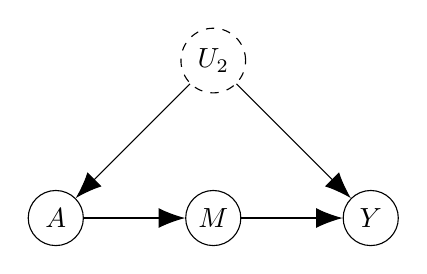
\begin{tikzpicture}[>=Stealth, node distance=2cm, on grid, auto]
  % Nodes
  \begin{scope}
 % \node (Z) [rv] {$Z$};
  \node (A) [rv] {$A$};
  \node (M) [right = of A, rv] {$M$};
  \node (Y) [right = of M, rv] {$Y$};
  % \node (V5) [below = of V2, rv, xshift=10mm, yshift=3mm] {$V_5$};
  %\node (U1) [right = of V1] {$U_1$};
  % \node (U1) [right = of V5] {$U_1$};
  \node[draw,circle,dashed] (U2) [above = of M] {$U_2$};
  
  
  % Arrows
 % \draw [-{Latex[scale=2.0]}] (Z) -- (A);
  \draw [-{Latex[scale=2.0]}] (A) -- (M);
  \draw [-{Latex[scale=2.0]}] (M) -- (Y);
  % \draw [-{Latex[scale=2.0]}] (V1) -- (V5);
  % Dashed arrows (unobserved variables)
  %\draw [-{Latex[scale=2.0]}] (U1) -- (V1);
  % \draw [-{Latex[scale=2.0]}] (U1) -- (V5);
  % \draw [-{Latex[scale=2.0]}] (U1) -- (V4);
  \draw [-{Latex[scale=2.0]}] (U2) -- (A);
  \draw [-{Latex[scale=2.0]}] (U2) -- (Y);
\end{scope}
\end{tikzpicture}
    \caption{Front door model.}
    \label{fig:frontdoorbase}
\end{figure}

When applying our algorithm to the front door model in Figure \ref{fig:frontdoorbase}, we get the following constraints reported as potentially nontrivial: 
\vspace{-0.5 cm}
\begin{eqnarray*}
&& -\Pr(A = 0) + \Pr(A = 0)\Pr(Y = 0|A = 0,M = 1) \leq 0 \\
&& \Pr(A = 0) + \Pr(A = 1)\Pr(Y = 0|A = 1,M = 1) \leq 1 \\  && \Pr(A = 0) - \Pr(A = 0)  =  0 \\
&& -\Pr(A = 0) - \Pr(A = 1) =  -1. 
\end{eqnarray*}
These have been simplified from the original form they were provided by the algorithm to allow them to fit easily on the page and clearly illustrate that they are trivial. The reason these are flagged as nontrivial is clear when written in terms of the interventional quantities that were tested by the algorithm: 
% \begin{eqnarray*}
% &&-\Pr(A = 0, Y = 0| \Do(M = 0)) - \Pr(A = 0, Y = 1| \Do(M = 0)) \\ &+& \Pr(A = 0, Y = 0| \Do(M = 1)) \leq 0 \\        &&\Pr(A = 0, Y = 0| \Do(M = 0)) + \Pr(A = 0, Y = 1| \Do(M = 0))\\ &+& \Pr(A = 1, Y = 0| \Do(M = 1)) \leq 1 \\           &&\Pr(A = 0, Y = 0| \Do(M = 0)) + \Pr(A = 0, Y = 1| \Do(M = 0)) \\ &-& \Pr(A = 0, Y = 0| \Do(M = 1)) - \Pr(A = 0, Y = 1| \Do(M = 1))  =  0 \\
% &&-\Pr(A = 0, Y = 0| \Do(M = 0)) - \Pr(A = 0, Y = 1| \Do(M = 0)) \\ &-& \Pr(A = 1, Y = 0| \Do(M = 1)) - \Pr(A = 1, Y = 1| \Do(M = 1))  =  -1. \\
% \end{eqnarray*}
\begin{align*}
&-\Pr(A = 0, Y = 0 \mid \Do(M = 0))
 - \Pr(A = 0, Y = 1 \mid \Do(M = 0)) \\
&\quad
 + \Pr(A = 0, Y = 0 \mid \Do(M = 1))
 \leq 0
\\[0.75ex]
&\Pr(A = 0, Y = 0 \mid \Do(M = 0))
 + \Pr(A = 0, Y = 1 \mid \Do(M = 0)) \\
&\quad
 + \Pr(A = 1, Y = 0 \mid \Do(M = 1))
 \leq 1
\\[0.75ex]
&\Pr(A = 0, Y = 0 \mid \Do(M = 0))
 + \Pr(A = 0, Y = 1 \mid \Do(M = 0)) \\
&\quad
 - \Pr(A = 0, Y = 0 \mid \Do(M = 1))
 - \Pr(A = 0, Y = 1 \mid \Do(M = 1))
 = 0
\\[0.75ex]
&-\Pr(A = 0, Y = 0 \mid \Do(M = 0))
 - \Pr(A = 0, Y = 1 \mid \Do(M = 0)) \\
&\quad
 - \Pr(A = 1, Y = 0 \mid \Do(M = 1))
 - \Pr(A = 1, Y = 1 \mid \Do(M = 1))
 = -1 .
\end{align*}
These are not observable constraints because fixing $M$ directly results in the constraint. However, translating them to the identifying functionals under the front door model, we obtain trivial constraints on any observed distribution. Thus, constraints flagged by the algorithm as potentially nontrivial should always be investigated manually whenever possible to verify that they are nontrivial. However, testing all flagged constraints or imposing them during estimation would not be incorrect because the flagged but trivial constraints do not impose any additional restrictions on the distribution. The tripartite Bell example in Subsection \ref{sec:tripart} illustrates a situation where it would be cumbersome to manually investigate all potentially nontrivial constraints. 

\section{Novel Examples}
\subsection{Sequential instrumental variables}

The model for this example is shown in Figure \ref{fig:seqiv}. This DAG satisfies Conditions \ref{A1}, \ref{A2}, and it has a c-degree of 1. There are three districts: $\{V_1\}, \{V_2, V_3, U_2\}, \{V_4, V_5, U_3\}$. Using standard d-separation criteria, we find the conditional independence relation $(V_1, V_2) \indep (V_4, V_5) \mid V_3$. Applying our Algorithm and then Proposition \ref{prop:nontrivial}, we find the nontrivial constraints below that are recognizable as two sets of the instrumental inequalities, one for each of the two districts with unobserved variables: 
\begin{eqnarray*}
\Pr(V_2 = 1, V_3 = 1 | V_1 = 0) + \Pr(V_2 = 1, V_3 = 0 | V_1 = 1) &\leq 1 \\
\Pr(V_2 = 1, V_3 = 0 | V_1 = 0) + \Pr(V_2 = 1, V_3 = 1 | V_1 = 1) &\leq 1 \\
\Pr(V_2 = 0, V_3 = 1 | V_1 = 0) + \Pr(V_2 = 0, V_3 = 0 | V_1 = 1) &\leq 1 \\
\Pr(V_2 = 0, V_3 = 0 | V_1 = 0) + \Pr(V_2 = 0, V_3 = 1 | V_1 = 1) &\leq 1 \\
\Pr(V_4 = 1, V_5 = 1 | V_3 = 0) + \Pr(V_4 = 1, V_5 = 0 | V_3 = 1) &\leq 1 \\
\Pr(V_4 = 1, V_5 = 0 | V_3 = 0) + \Pr(V_4 = 1, V_5 = 1 | V_3 = 1) &\leq 1 \\
\Pr(V_4 = 0, V_5 = 1 | V_3 = 0) + \Pr(V_4 = 0, V_5 = 0 | V_3 = 1) &\leq 1 \\
\Pr(V_4 = 0, V_5 = 0 | V_3 = 0) + \Pr(V_4 = 0, V_5 = 1 | V_3 = 1) &\leq 1.
\end{eqnarray*}




\subsection{Nested equivalent models with distinct inequalities}

\begin{figure}[ht]
    \centering
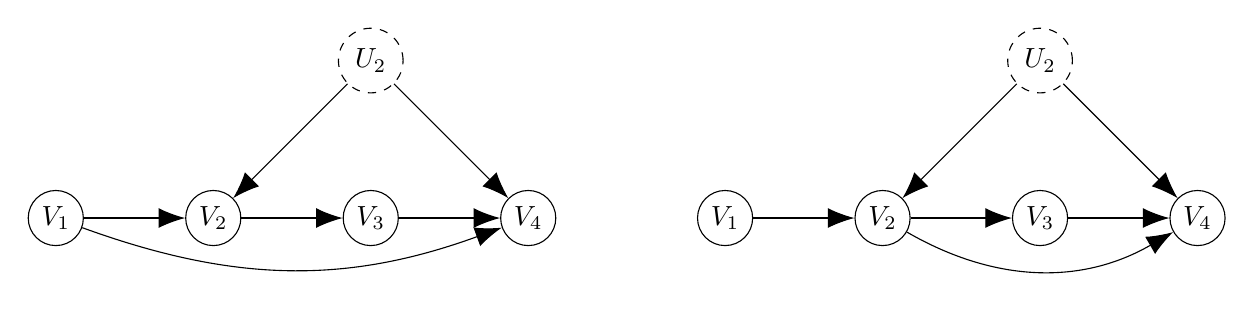
\begin{tikzpicture}[>=Stealth, node distance=2cm, on grid, auto]
  % Nodes
  \begin{scope}
  \node (V1) [rv] {$V_1$};
  \node (V2) [right = of V1, rv] {$V_2$};
  \node (V3) [right = of V2, rv] {$V_3$};
  \node (V4) [right = of V3, rv] {$V_4$};
  % \node (V5) [below = of V2, rv, xshift=10mm, yshift=3mm] {$V_5$};
  %\node (U1) [right = of V1] {$U_1$};
  % \node (U1) [right = of V5] {$U_1$};
  \node[draw,circle,dashed] (U2) [above = of V3] {$U_2$};
  
  
  % Arrows
  \draw [-{Latex[scale=2.0]}] (V1) -- (V2);
  \draw [-{Latex[scale=2.0]}] (V2) -- (V3);
  \draw [-{Latex[scale=2.0]}] (V3) -- (V4);
  % \draw [-{Latex[scale=2.0]}] (V1) -- (V5);
  \draw [-{Latex[scale=2.0]}] (V1) to[bend right=20] (V4);
  
  % Dashed arrows (unobserved variables)
  %\draw [-{Latex[scale=2.0]}] (U1) -- (V1);
  % \draw [-{Latex[scale=2.0]}] (U1) -- (V5);
  % \draw [-{Latex[scale=2.0]}] (U1) -- (V4);
  \draw [-{Latex[scale=2.0]}] (U2) -- (V4);
  \draw [-{Latex[scale=2.0]}] (U2) -- (V2);
\end{scope}
    

    \begin{scope}[xshift=8.5cm]
  \node (V1) [rv] {$V_1$};
  \node (V2) [right = of V1, rv] {$V_2$};
  \node (V3) [right = of V2, rv] {$V_3$};
  \node (V4) [right = of V3, rv] {$V_4$};
  % \node (V5) [below = of V2, rv, xshift=10mm, yshift=3mm] {$V_5$};
  %\node (U1) [right = of V1] {$U_1$};
  % \node (U1) [right = of V5] {$U_1$};
  \node[draw,circle,dashed] (U2) [above = of V3] {$U_2$};
  
  
  % Arrows
  \draw [-{Latex[scale=2.0]}] (V1) -- (V2);
  \draw [-{Latex[scale=2.0]}] (V2) -- (V3);
  \draw [-{Latex[scale=2.0]}] (V3) -- (V4);
  % \draw [-{Latex[scale=2.0]}] (V5) -- (V4);
  % \draw [-{Latex[scale=2.0]}] (V1) -- (V5);
  \draw [-{Latex[scale=2.0]}] (V2) to[bend right] (V4);

  % Dashed arrows (unobserved variables)
  %\draw [-{Latex[scale=2.0]}] (U1) -- (V1);
  % \draw [-{Latex[scale=2.0]}] (U1) -- (V5);
  % \draw [-{Latex[scale=2.0]}] (U1) -- (V4);
  \draw [-{Latex[scale=2.0]}] (U2) -- (V4);
  \draw [-{Latex[scale=2.0]}] (U2) -- (V2);
\end{scope}
\end{tikzpicture}
    \caption{Two graphs that are nested Markov equivalent, but which have distinct inequality constraints.}
    \label{fig:nested-ineq}
\end{figure}

Figure \ref{fig:nested-ineq} shows an example of two graphs that have the same sets of equality constraints (i.e., the same nested Markov model), but which differ when inequalities are also considered. Both graphs satisfy Conditions \ref{A1}, \ref{A2}, have c-degree 1, and have three districts: $\{V_1\}, \{V_2, V_4, U_2\}, \{V_3\}$. Both graphs imply that $V_1 \indep V_3 \mid V_2$. In both graphs, the districts $\{V_1\}$ and $\{V_3\}$ imply only trivial constraints. The interesting constraints are associated with the district $\{V_2, V_4, U_2\}$, and probabilities of the form
\begin{eqnarray*}
&& \Pdo(V_2 = v_2, V_4 = v_4 | V_1 = v_1, V_3 = v_3) = \\ 
&& \Pr(V_2 = v_2 | V_1 = v_1) \Pr(V_4 = v_4 | V_2 = v_2, V_1 = v_1, V_3 = v_3).   
\end{eqnarray*}

%Both graphs share the equality constraints of the form
%\begin{eqnarray*}
%&& \Pdo(V_2 = v_2 | V_1 = v_1, V_3 = v_3) = \Pdo(V_2 = v_2 | V_1 = v_1), 
%\end{eqnarray*}
%for $v_1, v_2, v_3 \in \{0, 1\}$, which we can recognize as a nested Markov independence \citep{evans2019smooth}.

%Both graphs also share the following inequality constraints
%\begin{eqnarray*}
% && \Pdo(V_2 = 0 | V_1 = 1, V_3 = 0) + \Pdo(V_2 = 1, V_4 = 0 | V_1 = 1, V_3 = 1) \leq 1 \\
% && \Pdo(V_2 = 0 | V_1 = 0, V_3 = 0) + \Pdo(V_2 = 1, V_4 = 0 | V_1 = 0, V_3 = 1) \leq 1 \\
% && \Pdo(V_2 = 1 | V_1 = 1, V_3 = 0) + \Pdo(V_2 = 0, V_4 = 0 | V_1 = 1, V_3 = 1) \leq 1 \\
% && \Pdo(V_2 = 1 | V_1 = 0, V_3 = 0) + \Pdo(V_2 = 0, V_4 = 0 | V_1 = 0, V_3 = 1) \leq 1. \\
%\end{eqnarray*}
The graph on the left does not have any nontrivial constraints aside from the conditional independence (though our Algorithm flags some as potentially nontrivial similar to the front door model). Note that the graph on the right is such that after intervening on $V_3$ we obtain an instrumental variable model over $V_1,V_2,V_4$ (for each level of $V_3$).  In contrast, the graph on the left is saturated over that margin. Therefore, we get some nontrivial inequality constraints in the right graph that are not present under the left graph. They are 
\begin{eqnarray*}
&& \Pdo(V_2 = 0, V_4 = 1 | V_1 = 0, V_3 = 0) + \Pdo(V_2 = 0, V_4 = 0 | V_1 = 1, V_3 = 0) \leq 1 \\
&& \Pdo(V_2 = 0, V_4 = 0 | V_1 = 0, V_3 = 0) + \Pdo(V_2 = 0, V_4 = 1 | V_1 = 1, V_3 = 0) \leq 1 \\
&& \Pdo(V_2 = 1, V_4 = 0 | V_1 = 0, V_3 = 0) + \Pdo(V_2 = 1, V_4 = 1 | V_1 = 1, V_3 = 0) \leq 1 \\ 
&& \Pdo(V_2 = 1, V_4 = 1 | V_1 = 0, V_3 = 0) + \Pdo(V_2 = 1, V_4 = 0 | V_1 = 1, V_3 = 0) \leq 1 \\ 
&& \Pdo(V_2 = 0 | V_1 = 1, V_3 = 0) + \Pdo(V_2 = 0, V_4 = 0 | V_1 = 0, V_3 = 1) \\ 
&& \quad - \Pdo(V_2 = 0, V_4 = 0 | V_1 = 1, V_3 = 1) \leq 1 \\ 
&& \Pdo(V_2 = 0 | V_1 = 0, V_3 = 0) + \Pdo(V_2 = 0, V_4 = 0 | V_1 = 1, V_3 = 1) \\ 
&& \quad - \Pdo(V_2 = 0, V_4 = 0 | V_1 = 0, V_3 = 1) \leq 1 \\ 
&& \Pdo(V_2 = 1 | V_1 = 1, V_3 = 0) + \Pdo(V_2 = 1, V_4 = 0 | V_1 = 0, V_3 = 1) \\ 
&& \quad - \Pdo(V_2 = 1, V_4 = 0 | V_1 = 1, V_3 = 1) \leq 1 \\ 
&& \Pdo(V_2 = 1 | V_1 = 0, V_3 = 0) + \Pdo(V_2 = 1, V_4 = 0 | V_1 = 1, V_3 = 1) \\ 
&& \quad - \Pdo(V_2 = 1, V_4 = 0 | V_1 = 0, V_3 = 1) \leq 1.
\end{eqnarray*}
Here we are writing the constraints in terms of the \emph{star} probabilities, which are equal to observable probabilities, because in this case they are more concise and make it easier to relate them to nested Markov constraints. 

\subsection{Tripartite Bell graphs} \label{sec:tripart}

\begin{figure}[ht]
\begin{center}
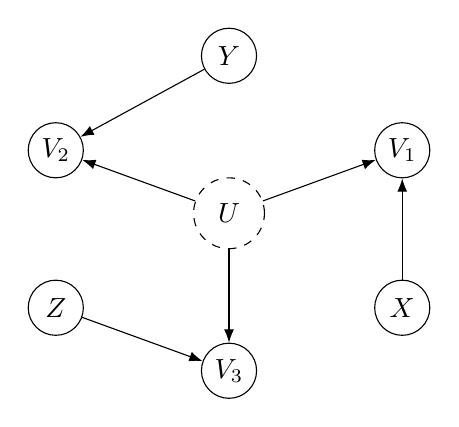
\begin{tikzpicture}[
    >=Latex,
    var/.style   ={draw,circle,minimum size=9mm,inner sep=0pt},
    latent/.style={draw,dashed,circle,minimum size=9mm,inner sep=0pt}
]
% Nodes (top row: X Y Z; bottom row: A B C; latent U centered above)
\node[latent]  (L) at (0,0)    {$U$};

\node[rv] (A) at ( 2.2, 0.8) {$V_1$};
\node[rv] (X) at ( 2.2,-1.2) {$X$};

\node[rv] (C) at ( 0.0,-2.0) {$V_3$};
\node[rv] (Z) at (-2.2,-1.2) {$Z$};

\node[rv] (B) at (-2.2, 0.8) {$V_2$};
\node[rv] (Y) at ( 0.0, 2.0) {$Y$};

% Arrows from settings to outcomes
\draw[->] (X) -- (A);
\draw[->] (Y) -- (B);
\draw[->] (Z) -- (C);

% Arrows from latent to outcomes
\draw[->] (L) -- (A);
\draw[->] (L) -- (B);
\draw[->] (L) -- (C);

\end{tikzpicture}
\end{center}
\caption{The tripartite Bell scenario. \label{fig:tripart}}
\end{figure}

Figure \ref{fig:tripart} is a well-known causal model in quantum physics. An incomplete set of constraints has been derived using the entropy method in \citet{bell3}. Our algorithm finds the complete set of constraints in this setting in less than 0.5 CPU-hours on a laptop running Ubuntu 22 with an AMD Ryzen 7 and 32 GB of RAM. First we identify the standard independencies $X \indep (V_2, V_3, Y, Z)$, $Y \indep (V_1, V_3, X, Z)$, and $Z \indep (V_1, V_2, X, Y)$. The subsequent part of the algorithm yields an additional 53,894 constraints total, out of which there are 53,856 inequality constraints, in agreement with \citet{Sliwa2003Symmetries} and \citet{Pironio_2011}. Our method further identifies 32,866 of those as potentially nontrivial constraints, 6 of which are equality constraints. The 6 equality constraints repeat the independence relations $(V_1, V_3) \indep Y$, $(V_1, V_2) \indep Z$, and $(V_2, V_3) \indep X$. An example of one of the inequality constraints, using the notation $\Pr(v_1 v_2 v_3 | xyz) = \Pr(V_1 = v_1, V_2 = v_2, V_3 = v_3 | X = x, Y = y, Z = z)$, is

\begin{align*}
& \Pr(001|010) + \Pr(010|101) - \Pr(110|001) - \Pr(010|100) - \\
& \Pr(000|111) - \Pr(001|000) - \Pr(011|000) \leq 0.
\end{align*}




\section{Extension to potentially incomplete linear constraints}
\label{sec:nonlin}
We extend our Algorithm to allow for DAGs with c-degree greater than 1. Prior to applying the Algorithm in Section \ref{algorithm}, for each district $D_j$:
\begin{enumerate}
    \item check that the c-degree of $D_j$ is at least $2$, otherwise pass through;
    \item create a new unobserved variable $U_j^*$; 
    \item if there exists an edge from any unobserved variable to $V_i$ in $D_j$, add an edge $U_j^* \rightarrow V_i$;
    \item then remove every unobserved variable (and its edges) other than $U_j^*$ from $D_j$. 
\end{enumerate}

\begin{remark}
\label{prop:merge}
Let $\mathcal{G}'$ be a DAG satisfying Conditions \ref{A1}, \ref{A2}, and with c-degree greater than 1. Let $\mathcal{G}$ be the causal model obtained from $\mathcal{G}'$ by merging unobserved variables so that the c-degree is 1. 
Then the constraints admitted by $\mathcal{G}$ hold under $\mathcal{G}'$.
\end{remark}

We now consider the two examples where our algorithm does not apply as discussed in Section \ref{sec:complete}.
Figure \ref{fig:incomp}, left side, shows an example DAG that also appears in  \citet{duarte2023automated}. This DAG has two districts, $\{V_1, V_3, V_6, U_2\}$ that has c-degree 1 and $\{V_2, V_4, V_5, U_1, U_3\}$ that has c-degree 2. It satisfies Conditions \ref{A1} and \ref{A2}, but since the c-degree is greater than 1, we cannot guarantee that the constraints derived by our algorithm are complete. In this case, we proceed by merging the unobserved variables $U_1$ and $U_3$ into a single unobserved variable $U_{13}$ that has child set equal to the union of the child sets of $U_1$ and $U_3$ (Figure \ref{fig:incomp}, right side). This converts the potentially nonlinear problem to a linear one. The constraints we obtain in these cases are still valid, but they are not necessarily complete. 


\begin{figure}[ht]
\begin{center}
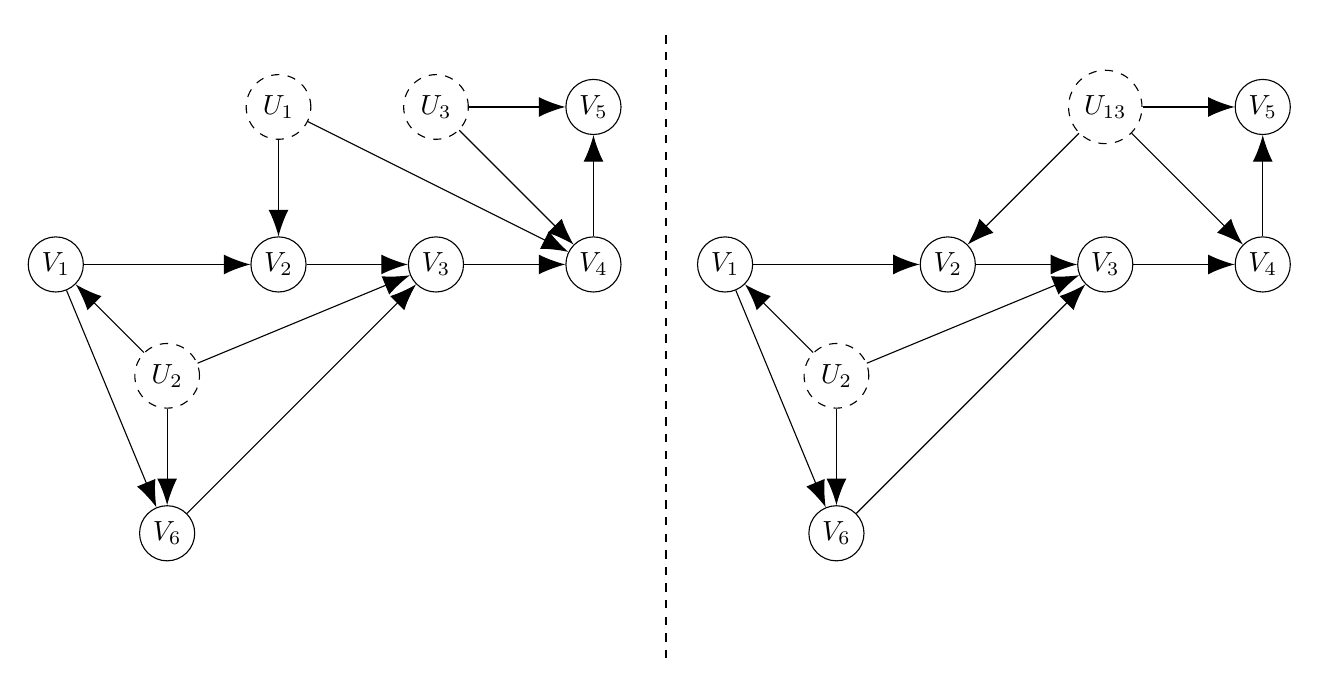
\begin{tikzpicture}[>=Stealth, node distance=2cm, on grid, auto]
\begin{scope}
  % Nodes
  \node (A) [rv] {$V_1$};
  \node[draw,circle,dashed] (U2) [below right= of A] {$U_2$};
  \node (B) [above right=of U2, rv] {$V_2$};
  \node (C) [right=of B, rv] {$V_3$};
  \node (D) [right=of C, rv] {$V_4$};
  
  \node (F) [above =of D, rv] {$V_5$};

  % unobserved variables (U1, U2, U3)
  \node[draw,circle,dashed] (U1) [above =of B] {$U_1$};
  
  \node[draw,circle,dashed] (U3) [above =of C] {$U_3$};
\node (E) [below=of U2, rv] {$V_6$};
  % Arrows
  \draw [-{Latex[scale=2.0]}]  (A) -- (B);
  \draw [-{Latex[scale=2.0]}]  (E) -- (C);
  \draw [-{Latex[scale=2.0]}]  (C) -- (D);
  \draw [-{Latex[scale=2.0]}]  (D) -- (F);
  \draw [-{Latex[scale=2.0]}]  (A) -- (E);
  \draw [-{Latex[scale=2.0]}]  (B) -- (C);

  % Dashed arrows (unobserved variables)
  \draw [-{Latex[scale=2.0]}] (U1) -- (B);
  \draw [-{Latex[scale=2.0]}] (U1) -- (D);
  \draw [-{Latex[scale=2.0]}] (U2) -- (A);
  \draw [-{Latex[scale=2.0]}] (U2) -- (E);
  \draw [-{Latex[scale=2.0]}] (U2) -- (C);
  \draw [-{Latex[scale=2.0]}] (U3) -- (F);
  \draw [-{Latex[scale=2.0]}] (U3) -- (D);
   \draw[dashed] (7.75, -5) -- (7.75, 3);
\end{scope}
\begin{scope}[xshift=8.5cm]
  \node (A) [rv] {$V_1$};
  \node[draw,circle,dashed] (U2) [below right= of A] {$U_2$};
  \node (B) [above right=of U2, rv] {$V_2$};
  \node (C) [right=of B, rv] {$V_3$};
  \node (D) [right=of C, rv] {$V_4$};
  
  \node (F) [above =of D, rv] {$V_5$};

  % unobserved variables (U1, U2, U3)
  %\node[draw,circle,dashed] (U1) [above =of B] {$U_1$};
  
  \node[draw,circle,dashed] (U13) [above =of C] {$U_{13}$};
\node (E) [below=of U2, rv] {$V_6$};
  % Arrows
  \draw [-{Latex[scale=2.0]}]  (A) -- (B);
  \draw [-{Latex[scale=2.0]}]  (E) -- (C);
  \draw [-{Latex[scale=2.0]}]  (C) -- (D);
  \draw [-{Latex[scale=2.0]}]  (D) -- (F);
  \draw [-{Latex[scale=2.0]}]  (A) -- (E);
  \draw [-{Latex[scale=2.0]}]  (B) -- (C);

  % Dashed arrows (unobserved variables)
  \draw [-{Latex[scale=2.0]}] (U13) -- (B);
  \draw [-{Latex[scale=2.0]}] (U13) -- (D);
  \draw [-{Latex[scale=2.0]}] (U2) -- (A);
  \draw [-{Latex[scale=2.0]}] (U2) -- (E);
  \draw [-{Latex[scale=2.0]}] (U2) -- (C);
  \draw [-{Latex[scale=2.0]}] (U13) -- (F);
\end{scope}
\end{tikzpicture}
\end{center}
\caption{Example model with two districts and c-degree 2 (left side), and the model after merging the unobserved variables $U_1$ and $U_3$ to make the c-degree 1 (right side). \label{fig:incomp}}
\end{figure}

For the first district in the graph in Figure \ref{fig:incomp} that contains $V_1, V_3, V_6$, we find 8 possibly nontrivial constraints, 4 inequality and 4 equality constraints. The equality constraints are again strictly nested Markov independences that state $\Pdo(V_1 = v_1, V_6 = v_6| V_2 = v_2) = \Pdo(V_1 = v_1 | V_2 = v_2)$, while the inequality constraints take the form 
\[
\Pdo(V_1 = 0, V_3 = 0, V_6 = 0| V_2 = 1) \leq \Pdo(V_1 = 0, V_6 = 0| V_2 = 0),
\]
for different levels of $V_1, V_3, V_6$.

After merging $U_1$ and $U_3$ in the second district and applying our algorithm, we find 1118 potentially nontrivial constraints. In the interest of space, we do not reproduce them here, but given an observed distribution, it is straightforward to check whether they are violated or not using the matrix representations of the constraints. 

This process of merging latent variables to create a DAG with c-degree 1 can be applied as a pre-processing step before using our Algorithm to obtain some constraints in more general settings, but again this does not necessarily yield the complete constraints. In words, for models that have more than one unobserved variable in at least one district, the constraints obtained by our Algorithm are necessary but not necessarily complete. That is, they must hold but there may be more constraints than the linear ones we are able to derive. 

We now consider the Triangle scenario. If we merge the three unobserved variables into a single common parent of all three observable variables, which is depicted in the right side of Figure \ref{fig:triangle}, we can apply our algorithm. Our algorithm does not produce any nontrivial constraints that can witness incompatibility. In this case, we know that this set of constraints is incomplete, because of the nontrivial constraints presented in \citet{Wolfe_2019} for this setting. 

\begin{figure}[ht]
\begin{center}
   \begin{tikzpicture}[
    >=Latex,
    rv/.style   ={draw,circle,minimum size=9mm,inner sep=0pt},
    latent/.style={draw,dashed,circle,minimum size=9mm,inner sep=0pt}
]
\begin{scope}
% Positions (roughly circular layout)
%\node[latent]  (L) at (0,0)    {$\lambda$};

\node[rv] (A) at ( 2.2, 0.8) {$V_1$};
\node[latent] (X) at ( 2.2,-1.2) {$U_1$};

\node[rv] (C) at ( 0.0,-2.0) {$V_3$};
\node[latent] (Z) at (-2.2,-1.2) {$U_3$};

\node[rv] (B) at (-2.2, 0.8) {$V_2$};
\node[latent] (Y) at ( 0.0, 2.0) {$U_2$};

% Arrows from settings to outcomes
\draw[->] (X) -- (A);
\draw[->] (Y) -- (B);
\draw[->] (Z) -- (C);

% Arrows from latent to outcomes
\draw[->] (X) -- (C);
\draw[->] (Y) -- (A);
\draw[->] (Z) -- (B);
 \draw[dashed] (4.5, -3) -- (4.5, 3);
\end{scope}
\begin{scope}[xshift=8.5cm]
% Positions (roughly circular layout)
%\node[latent]  (L) at (0,0)    {$\lambda$};

\node[rv] (A) at ( 2.2, 0.8) {$V_1$};
\node[latent] (X) at ( 0,0) {$U$};

\node[rv] (C) at ( 0.0,-2.0) {$V_3$};
%\node[latent] (Z) at (-2.2,-1.2) {$U_3$};

\node[rv] (B) at (-2.2, 0.8) {$V_2$};
%\node[latent] (Y) at ( 0.0, 2.0) {$U_2$};

% Arrows from settings to outcomes
\draw[->] (X) -- (A);
\draw[->] (X) -- (B);
\draw[->] (X) -- (C);

\end{scope}
\end{tikzpicture}
\end{center}
\caption{The triangle scenario (left) and the graph obtained by merging the three unobserved variables into one.}
    \label{fig:triangle}
\end{figure}

\section{Observationally equivalent DAGs} \label{graphmod}
Multiple graphs may be observationally equivalent and therefore admit the same set of constraints. For example, the graph $X \rightarrow Y$ is observationally equivalent to the graph where $X$ and $Y$ share an unobserved parent.
Proposition 5 of \citet{evans2016graphs} and its extensions \citep{ansanelli2025observationalpartialordercausal} can be used to obtain graphs with lower c-degree that are observationally equivalent to graphs with c-degree greater than one. We note that DAGs obtained with these results may not be causally equivalent, but are \emph{observationally} equivalent to the DAG under study. The following Proposition \ref{prop:replace} provides a recipe for converting between observationally equivalent DAGs that may have different c-degrees. %Thus we translate this result to our notation and hidden variable DAGs for the purposes of reducing the number of unobserved variables within a district. 

\begin{proposition}[Evans 2016] \label{prop:replace}
Let $\mathcal{G}$ be a DAG that meets Conditions \ref{A1} and \ref{A2}, and $\boldsymbol{C}, \boldsymbol{D}$ be disjoint sets of observed vertices. If 
\begin{itemize}
    \item $\boldsymbol{C} \cup \boldsymbol{D} = \Chobs(U_i)$; 
    \item $c \notin \Chobs(U_j)$ for all $c \in \boldsymbol{C}$, for any other unobserved vertex $U_j \neq U_i$;
    \item $\Pa(\boldsymbol{C}) \subseteq\Pa(d)$ for every $d \in \boldsymbol{D}$;
\end{itemize}
then the graph obtained by replacing every path of the form $c \leftarrow U_i \rightarrow d$ with $c \rightarrow d$ for every pair $c \in \boldsymbol{C}$, $d \in \boldsymbol{D}$ has the same constraints as $\mathcal{G}$.

\end{proposition}

The Henson-Lal-Pusey \citep{henson2014theory} result provides conditions under which one can add an edge to a DAG without changing the constraints.

\begin{proposition}[HLP Proposition] \label{prop:hlp}
  Let $\mathcal{G}$ be a DAG that meets Conditions \ref{A1} and \ref{A2}, and $V_1$ and $V_2$ observed nodes.  
  If: 
  \begin{itemize}
      \item $\Pa(V_1) \subseteq \Pa(V_2)$;
      % \item $W_1$ is included in at least one hyperedge;
      \item There exists a $U_1$ s.t. $\{V_1, V_2\} \subseteq \Chobs(U_1)$ ;
  \end{itemize}
  then the graph has the same constraints as the one in which, in addition, we have the edge $V_1 \to V_2$.
\end{proposition}

Combining the HLP proposition with the following result from \citet{ansanelli2025observationalpartialordercausal} (adapted to our notation) can show observational equivalences in cases where Proposition \ref{prop:replace} cannot, and subsumes Proposition \ref{prop:replace}. We include Proposition \ref{prop:replace} because it may be easier to recognize situations where it can be applied. 

\begin{proposition}[Strong Face Splitting] \label{prop:strong}
  Let $\mathcal{G}$ be a DAG meeting Conditions \ref{A1} and \ref{A2}, containing the following unobserved vertices 
  $U_1,\ldots,U_k$ that share $D = \bigcap_{i=1}^k \Chobs(U_i)$.  Let $C_i = \Chobs(U_i) \setminus D$. If the following conditions hold:
  \begin{itemize}
      \item $\Pa(C_i) \cup C_i \subseteq \Pa(d)$ for each $d \in D$, for $i = 1, \dots, k$;
      \item if for an unobserved vertex $U_j$, we have $c \in \Chobs(U_j)$ for some $c \in \bigcup_{i=1}^k C_i$ then $D \subseteq \Chobs(U_j)$;
  \end{itemize}
  then the DAG obtained from the observed subgraph of $\mathcal{G}$, adding the unobserved vertices $U^*_1, \ldots, U^*_k, U^*_{k+1}$ and corresponding edges $\{U^*_1 \rightarrow c: c \in C_1\}, \ldots, \{U^*_k \rightarrow c: c \in C_k\}, \{U^*_{k+1} \rightarrow d: d \in D\}$ has the same constraints as $\mathcal{G}$.
\end{proposition}

A simple example of using these results is shown in Figure \ref{fig:ivequiv}. The three DAGs are known to be observationally equivalent, but our method applies only to the rightmost DAG because it has c-degree one. Thus our method can provide complete constraints in settings with c-degree greater than one, for any DAG that can be converted via Proposition \ref{prop:replace} or Propositions \ref{prop:hlp} and \ref{prop:strong} to a DAG with c-degree one. 


\begin{figure}[ht]
\centering

    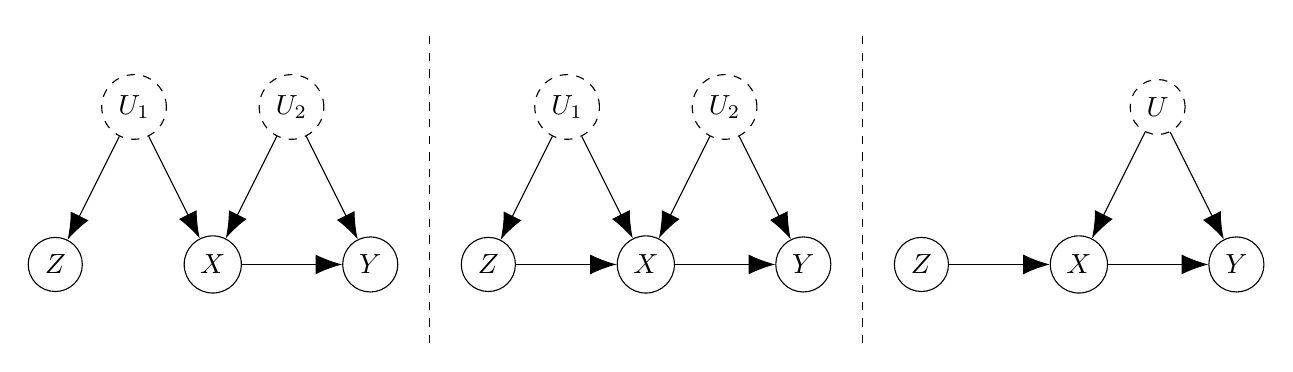
\begin{tikzpicture}
    \begin{scope}[xshift=-2cm]
      \node[draw, circle] at (2, 0) (X) {\(X\)};
    \node[draw, circle] at (4, 0) (Y) {\(Y\)};
    \node[draw, circle] at (0, 0) (Z) {$Z$};
    %\node[draw, circle] at (-3, 4) (S) {\(S\)};
   % \node[draw, circle] at (-4, 0) (Z) {\(Z\)};
    \node[draw, circle, dashed] at (1,2) (U1) {\(U_1\)};
    \node[draw, circle, dashed] at (3,2) (U2) {\(U_2\)};
   \draw [-{Latex[scale=2.0]}] (X) to (Y);
   % \draw [-{Latex[scale=2.0]}] (Z) to (X);
    %\draw [-{Latex[scale=2.0]}] (S) to (X);
    %\draw [-{Latex[scale=2.0]}] (S) to (Y);
    \draw [-{Latex[scale=2.0]}] (U2) to (X);
    \draw [-{Latex[scale=2.0]}] (U2) to (Y);
    \draw [-{Latex[scale=2.0]}] (U1) to (X);
    \draw [-{Latex[scale=2.0]}] (U1) to (Z);
   %
   % \draw [-{Latex[scale=2.0]}] (Z) to (X);
    %\draw [-, dashed] (S) to (U);
    \draw[dashed] (4.75, -1) -- (4.75, 3);

    \end{scope}% Nodes
\begin{scope}[xshift=3.5cm]
 
  \node[draw, circle] at (2, 0) (X) {\(X\)};
    \node[draw, circle] at (4, 0) (Y) {\(Y\)};
    \node[draw, circle] at (0, 0) (Z) {$Z$};
    %\node[draw, circle] at (-3, 4) (S) {\(S\)};
   % \node[draw, circle] at (-4, 0) (Z) {\(Z\)};
    \node[draw, circle, dashed] at (1,2) (U1) {\(U_1\)};
    \node[draw, circle, dashed] at (3,2) (U2) {\(U_2\)};
   \draw [-{Latex[scale=2.0]}] (X) to (Y);
    \draw [-{Latex[scale=2.0]}] (Z) to (X);
    %\draw [-{Latex[scale=2.0]}] (S) to (X);
    %\draw [-{Latex[scale=2.0]}] (S) to (Y);
    \draw [-{Latex[scale=2.0]}] (U2) to (X);
    \draw [-{Latex[scale=2.0]}] (U2) to (Y);
    \draw [-{Latex[scale=2.0]}] (U1) to (X);
    \draw [-{Latex[scale=2.0]}] (U1) to (Z);
    \draw[dashed] (4.75, -1) -- (4.75, 3);

    \end{scope}% Nodes
    
  \begin{scope}[xshift=9cm] 
    
  
   % \draw [-{Latex[scale=2.0]}] (Z) to (X);
    %\draw [-, dashed] (S) to (U);
   \node[draw, circle] at (2, 0) (X) {\(X\)};
    \node[draw, circle] at (4, 0) (Y) {\(Y\)};
    \node[draw, circle] at (0, 0) (Z) {$Z$};
    %\node[draw, circle] at (-3, 4) (S) {\(S\)};
   % \node[draw, circle] at (-4, 0) (Z) {\(Z\)};
    \node[draw, circle, dashed] at (3,2) (U) {\(U\)};
    \draw [-{Latex[scale=2.0]}] (X) to (Y);
    \draw [-{Latex[scale=2.0]}] (Z) to (X);
    %\draw [-{Latex[scale=2.0]}] (S) to (X);
    %\draw [-{Latex[scale=2.0]}] (S) to (Y);
    \draw [-{Latex[scale=2.0]}] (U) to (X);
    \draw [-{Latex[scale=2.0]}] (U) to (Y);
   % \draw [-{Latex[scale=2.0]}] (Z) to (X);
    %\draw [-, dashed] (S) to (U);
   

  \end{scope}
    \end{tikzpicture}
  
    \caption{\label{fig:ivequiv} A DAG with c-degree two (left). Applying the HLP Proposition, we get the center DAG that has equivalent constraints. Applying Strong Face Splitting to the center DAG, we get the observationally equivalent classic IV DAG on the right that has c-degree one. Equivalently, we can apply Proposition \ref{prop:replace} to the left and center DAGs with $\boldsymbol{C} = \{Z\}$ and $\boldsymbol{D} = \{X\}$.}
    \end{figure}  


The example in Figure \ref{fig:propstrong} illustrates two graphs that Proposition \ref{prop:strong} can be used to show the equivalence of, but Proposition \ref{prop:replace} cannot. The original DAG has a single district with c-degree two. Applying the Strong Face Splitting result in combination with the HLP Proposition, we obtain an observationally equivalent DAG with two districts, one with c-degree one and one with c-degree two. This is merely to demonstrate that there are settings where Strong Face Splitting in addition to the HLP Proposition can show equivalence where Proposition \ref{prop:replace} cannot. Proposition 5 or Strong Face Splitting in combination with the HLP Proposition could once again be applied to the resulting graph to further reduce the c-degree, as shown in the bottom of Figure \ref{fig:propstrong}. The observationally equivalent DAG with c-degree zero in the bottom right of the Figure does not imply any conditional independencies based on d-separation, hence we find that there are no nontrivial constraints in the original DAG. 


\begin{figure}[ht]
\centering

    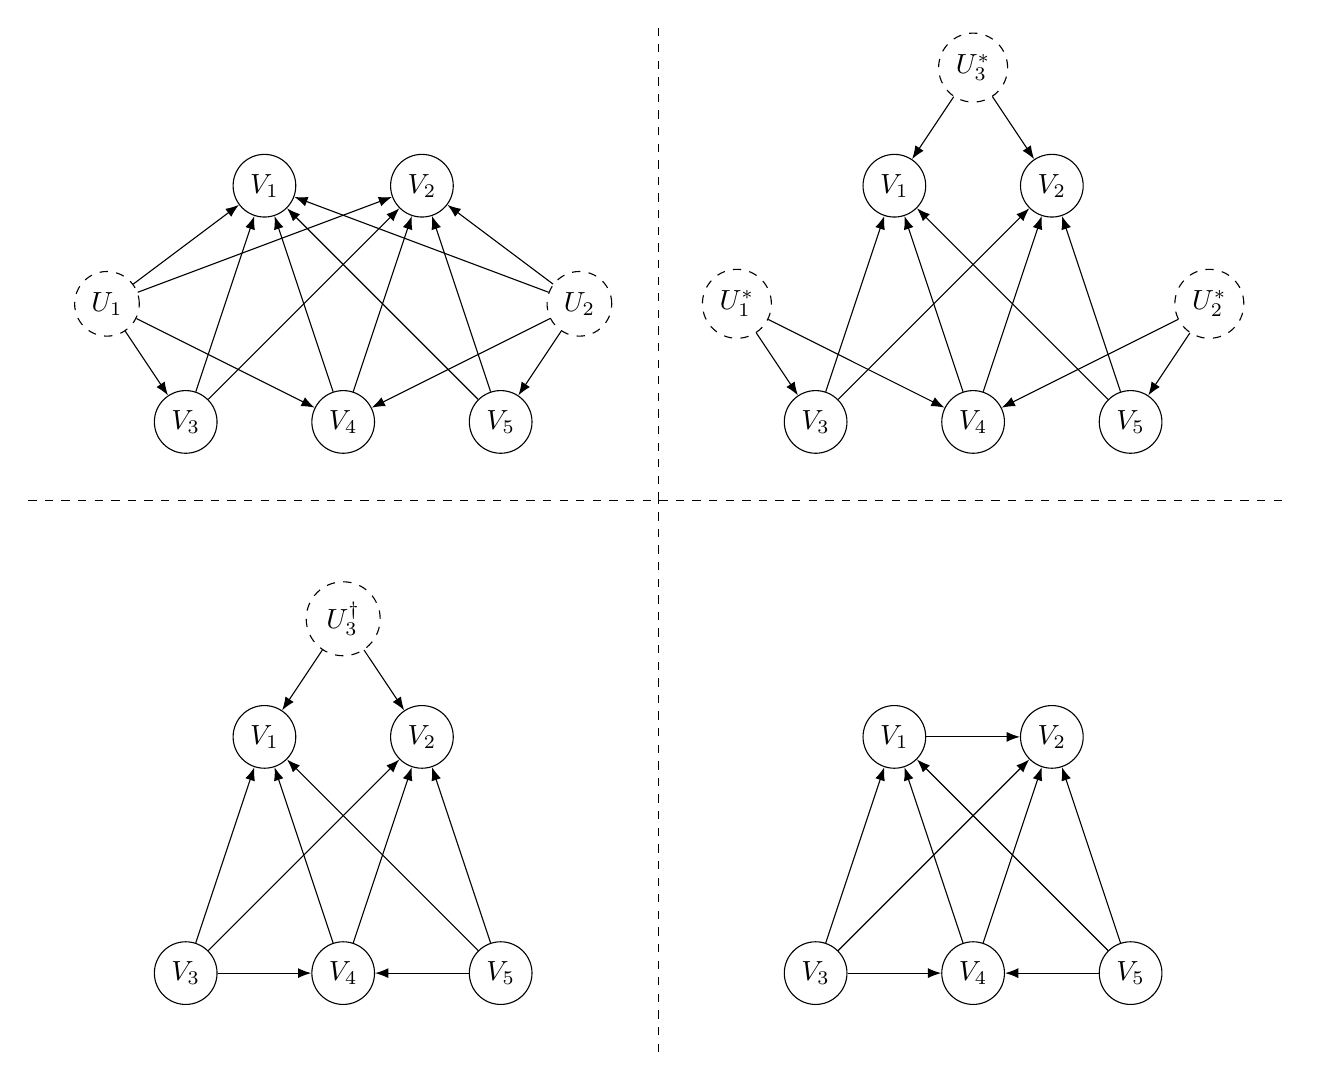
\begin{tikzpicture}
    
\begin{scope}[xshift=-2cm]
 
  \node[draw, circle] at (1, 3) (V1) {$V_1$};
    \node[draw, circle] at (3, 3) (V2) {$V_2$};
    \node[draw, circle] at (0, 0) (V3) {$V_3$};
    \node[draw, circle] at (2, 0) (V4) {$V_4$};
    \node[draw, circle] at (4, 0) (V5) {$V_5$};
    
    \node[draw, circle, dashed] at (-1,1.5) (U1) {\(U_1\)};
    \node[draw, circle, dashed] at (5,1.5) (U2) {\(U_2\)};
   \draw [-{Latex[scale=1.0]}] (V3) to (V1);
   \draw [-{Latex[scale=1.0]}] (V4) to (V1);
   \draw [-{Latex[scale=1.0]}] (V5) to (V1);
   \draw [-{Latex[scale=1.0]}] (V3) to (V2);
   \draw [-{Latex[scale=1.0]}] (V4) to (V2);
   \draw [-{Latex[scale=1.0]}] (V5) to (V2);
   \draw [-{Latex[scale=1.0]}] (U1) to (V1);
   \draw [-{Latex[scale=1.0]}] (U1) to (V2);
   \draw [-{Latex[scale=1.0]}] (U1) to (V3);
   \draw [-{Latex[scale=1.0]}] (U1) to (V4);
   \draw [-{Latex[scale=1.0]}] (U2) to (V1);
   \draw [-{Latex[scale=1.0]}] (U2) to (V2);
   \draw [-{Latex[scale=1.0]}] (U2) to (V5);
   \draw [-{Latex[scale=1.0]}] (U2) to (V4);
    \draw[dashed] (6, -1) -- (6, 5);
 \draw[dashed] (-2, -1) -- (14, -1);
    \end{scope}% Nodes
    
  \begin{scope}[xshift=6cm] 
    
  \node[draw, circle] at (1, 3) (V1) {$V_1$};
    \node[draw, circle] at (3, 3) (V2) {$V_2$};
    \node[draw, circle] at (0, 0) (V3) {$V_3$};
    \node[draw, circle] at (2, 0) (V4) {$V_4$};
    \node[draw, circle] at (4, 0) (V5) {$V_5$};
    
  \node[draw, circle, dashed] at (-1,1.5) (U1) {\(U^*_1\)};
    \node[draw, circle, dashed] at (5,1.5) (U2) {\(U^*_2\)};
    \node[draw, circle, dashed] at (2,4.5) (U3) {\(U^*_3\)};
     %\draw [-{Latex[scale=1.0]}] (V1) to (V2);
   \draw [-{Latex[scale=1.0]}] (V3) to (V1);
   \draw [-{Latex[scale=1.0]}] (V4) to (V1);
   \draw [-{Latex[scale=1.0]}] (V5) to (V1);
   \draw [-{Latex[scale=1.0]}] (V3) to (V2);
   %\draw [-{Latex[scale=1.0]}] (V3) to (V4);
   \draw [-{Latex[scale=1.0]}] (V4) to (V2);
   \draw [-{Latex[scale=1.0]}] (V5) to (V2);
   %\draw [-{Latex[scale=1.0]}] (V5) to (V4);
   \draw [-{Latex[scale=1.0]}] (U3) to (V1);
   \draw [-{Latex[scale=1.0]}] (U3) to (V2);
     \draw [-{Latex[scale=1.0]}] (U1) to (V3);
   \draw [-{Latex[scale=1.0]}] (U1) to (V4);
  \draw [-{Latex[scale=1.0]}] (U2) to (V5);
   \draw [-{Latex[scale=1.0]}] (U2) to (V4);
   

  \end{scope}

     
  \begin{scope}[xshift=-2cm, yshift=-7cm] 
    
  \node[draw, circle] at (1, 3) (V1) {$V_1$};
    \node[draw, circle] at (3, 3) (V2) {$V_2$};
    \node[draw, circle] at (0, 0) (V3) {$V_3$};
    \node[draw, circle] at (2, 0) (V4) {$V_4$};
    \node[draw, circle] at (4, 0) (V5) {$V_5$};
    
  %\node[draw, circle, dashed] at (-1,1.5) (U1) {\(U^*_1\)};
   % \node[draw, circle, dashed] at (5,1.5) (U2) {\(U^*_2\)};
    \node[draw, circle, dashed] at (2,4.5) (U3) {\(U^\dagger_3\)};
     %\draw [-{Latex[scale=1.0]}] (V1) to (V2);
   \draw [-{Latex[scale=1.0]}] (V3) to (V1);
   \draw [-{Latex[scale=1.0]}] (V4) to (V1);
   \draw [-{Latex[scale=1.0]}] (V5) to (V1);
   \draw [-{Latex[scale=1.0]}] (V3) to (V2);
   %\draw [-{Latex[scale=1.0]}] (V3) to (V4);
   \draw [-{Latex[scale=1.0]}] (V4) to (V2);
   \draw [-{Latex[scale=1.0]}] (V5) to (V2);
   %\draw [-{Latex[scale=1.0]}] (V5) to (V4);
   \draw [-{Latex[scale=1.0]}] (U3) to (V1);
   \draw [-{Latex[scale=1.0]}] (U3) to (V2);
%     \draw [-{Latex[scale=1.0]}] (U1) to (V3);
%   \draw [-{Latex[scale=1.0]}] (U1) to (V4);
%  \draw [-{Latex[scale=1.0]}] (U2) to (V5);
%   \draw [-{Latex[scale=1.0]}] (U2) to (V4);
   \draw [-{Latex[scale=1.0]}] (V3) to (V4);
   \draw [-{Latex[scale=1.0]}] (V5) to (V4);
   \draw[dashed] (6, -1) -- (6, 6);

  \end{scope}
  \begin{scope}[xshift=6cm, yshift=-7cm] 
    
  \node[draw, circle] at (1, 3) (V1) {$V_1$};
    \node[draw, circle] at (3, 3) (V2) {$V_2$};
    \node[draw, circle] at (0, 0) (V3) {$V_3$};
    \node[draw, circle] at (2, 0) (V4) {$V_4$};
    \node[draw, circle] at (4, 0) (V5) {$V_5$};
    
  %\node[draw, circle, dashed] at (-1,1.5) (U1) {\(U^*_1\)};
   % \node[draw, circle, dashed] at (5,1.5) (U2) {\(U^*_2\)};
   % \node[draw, circle, dashed] at (2,4.5) (U3) {\(U^\dagger_3\)};
     %\draw [-{Latex[scale=1.0]}] (V1) to (V2);
   \draw [-{Latex[scale=1.0]}] (V3) to (V1);
   \draw [-{Latex[scale=1.0]}] (V4) to (V1);
   \draw [-{Latex[scale=1.0]}] (V5) to (V1);
   \draw [-{Latex[scale=1.0]}] (V3) to (V2);
   \draw [-{Latex[scale=1.0]}] (V1) to (V2);
   %\draw [-{Latex[scale=1.0]}] (V3) to (V4);
   \draw [-{Latex[scale=1.0]}] (V4) to (V2);
   \draw [-{Latex[scale=1.0]}] (V5) to (V2);
   %\draw [-{Latex[scale=1.0]}] (V5) to (V4);
  % \draw [-{Latex[scale=1.0]}] (U3) to (V1);
 %  \draw [-{Latex[scale=1.0]}] (U3) to (V2);
%     \draw [-{Latex[scale=1.0]}] (U1) to (V3);
%   \draw [-{Latex[scale=1.0]}] (U1) to (V4);
%  \draw [-{Latex[scale=1.0]}] (U2) to (V5);
%   \draw [-{Latex[scale=1.0]}] (U2) to (V4);
   \draw [-{Latex[scale=1.0]}] (V3) to (V4);
   \draw [-{Latex[scale=1.0]}] (V5) to (V4);
   

  \end{scope}
    \end{tikzpicture}
  
    \caption{An example DAG (top left) where Proposition \ref{prop:strong} can be applied to show observational equivalence to the top right DAG, but not Proposition \ref{prop:replace}. Proposition \ref{prop:hlp} is then applied to the top right DAG to obtain the bottom left DAG that has c-degree 1. Finally Proposition \ref{prop:replace} is applied to the bottom left to obtain the bottom right DAG that has no hidden variables, wherein the lack of constraints can be seen directly based on the lack of d-separation. \label{fig:propstrong}}
    \end{figure}  

In the case of Figure \ref{fig:incomp}, we cannot apply either of these Propositions to reduce the c-degree. Consider the district containing $\{V_2,V_4,V_5\}$ that has c-degree two. In order to reduce the c-degree by removing $U_1$, we would need $V_2 \in \boldsymbol{C}$. Since $V_1$ is a parent of $V_2$ but not of $V_4$ nor $V_5$, the first condition of Proposition \ref{prop:replace} cannot be satisfied. We also cannot remove $U_3$ or $U_1$ using Strong Face Splitting because the parent set of $V_4$ does not contain the parents of $V_2$, and $V_2$ is not a parent of $V_4$.  


\section{Conclusion}

\citet{bonet2001instrumentality} observed that the complete set of observable constraints in the instrumental variables model can be derived with tools from computational geometry. We have extended this observation to a much broader class of causal models with unobserved variables, showing that a similar set of tools can be used to derive the complete set of equality and inequality constraints for any graph of c-degree one. Several of our examples illustrate that this method includes nontrivial equality constraints, similar to the Verma constraints or nested Markov constraints. However, unlike the constraints derived from the nested Markov model, our derived set of constraints may also include inequality constraints. 
%To distinguish this class of constraints from the previous equality-only nested Markov ones, we suggest the name MERA constraints, particularly when the set of constraints contain both equalities and inequalities and are complete. %Though we use the do operator and refer to causal models throughout, our results do not depend on giving a causal interpretation to a DAG and associated NPSEM-IE. 

The method is limited to DAGs with finite and discrete observed variables, though no assumptions are made about the state space of the unobserved variables. The method of deriving the constraints can be computationally demanding, as the number of facets of the polytope grows superexponentially in the number of variables. The precise complexity of the algorithm depends on the connectivity of the DAG, and the method can be computationally simple in graphs with many variables if they reside in different districts with simple connections between districts. It may be possible to adapt multithreaded implementations of computational geometry algorithms to perform this task \citep{Normaliz}, or to extend the pruning approach of \citet{shridharan2023scalable} to this setting to reduce the size of the linear program in certain cases. However, once derived for a given DAG, they are symbolic expressions that can be applied to any dataset or distribution. 

This method has potential applications in causal discovery with hidden variables, as this provides a finer stratification of causal models into equivalence classes than does independence testing or equality constraints alone. How to most effectively incorporate these constraints in causal discovery algorithms is an open question. These constraints also have potential applications in constrained statistical inference and partial identification.




\bibliographystyle{abbrvnat}
\bibliography{references.bib}

\end{document}
